%% Paper: Textualism as an effort-accuracy trade-off in rule enforcement
\documentclass[pdflatex,sn-nature]{sn-jnl}

%%%% Standard Packages
\usepackage{graphicx}%
\usepackage{multirow}%
\usepackage{amsmath,amssymb,amsfonts}%
\usepackage{amsthm}%xw
\usepackage{mathrsfs}%
\usepackage[title]{appendix}%
\usepackage{xcolor}%
\usepackage{textcomp}%
\usepackage{manyfoot}%
\usepackage{booktabs}%
\usepackage{url}
\urlstyle{same}  % or tt, rm, sf
\usepackage{xurl}
\usepackage{algorithm}%
\usepackage{algorithmicx}%
\usepackage{algpseudocode}%
\usepackage{listings}%
\usepackage{placeins}     % provides \FloatBarrier
\graphicspath{{./}}

\raggedbottom

\begin{document}

%%=============================================================%%
%% Title
%%=============================================================%%

\title[Textualism as an effort-accuracy trade-off]{Textualism as an effort-accuracy trade-off in rule enforcement}

%%=============================================================%%
%% Authors – fill in names, affiliations and emails
%%=============================================================%%

\author*[1]{\fnm{Ivar} \spfx{R.} \sur{Hannikainen}}\email{ivar@ugr.es}

\author[2]{\fnm{Neele} \sur{Engelmann}}\email{engelmann@mpib-berlin.mpg.de}

\author[3]{\fnm{Carlos} \sur{González-García}}\email{cgonzalez@ugr.es}

\author[3]{\fnm{María} \sur{Ruz}}\email{mruz@ugr.es}

\affil*[1]{\orgdiv{Department of Philosophy I}, \orgname{University of Granada}, \orgaddress{\city{Granada}, \postcode{18011}, \country{Spain}}}

\affil[2]{\orgdiv{Center for Humans and Machines}, \orgname{Max Planck Institute for Human Development}, \orgaddress{\city{Berlin}, \postcode{14195}, \country{Germany}}}

\affil[3]{\orgdiv{Mind, Brain and Behavior Research Center (CIMCYC)}, \orgname{University of Granada}, \orgaddress{\city{Granada}, \postcode{18071}, \country{Spain}}}

%%=============================================================%%
%% Abstract
%%=============================================================%%

\abstract{People often apply rules according to their letter even when doing so undermines their deeper spirit. Why does textualist enforcement prevail over competing approaches? We show that dilemmas that pit a rule's letter against its spirit elicit cognitive conflict, and examine whether their textualist resolution arises from improved deliberation or through experience. Challenging the deliberation model, inducing response caution did not influence interpretive approaches. However, prior task experience, and even exogenous cognitive demands, did promote textualist enforcement. Drift diffusion modeling indicated that this shift enabled a less effortful resolution of rule enforcement dilemmas through faster accumulation of textual evidence and reductions in the evidence threshold. Thus, we propose that textualism emerges as an adaptation to the cognitive labor of rule enforcement, reducing mental effort while preserving accuracy on low-conflict cases.}

\keywords{bounded rationality, computational modeling, cognitive control, letter vs. spirit, legal interpretation}

\maketitle

%%=============================================================%%
\section{Introduction}\label{sec:intro}
%%=============================================================%%

You download and fill out the required form, sign it and submit a scanned version only to discover that your application has been rejected on account of Article 3, which states: ``To ensure correct and complete information, applicants must submit an original signed form''. Why would the administrative assistant reject your application? One possible answer is that they are just applying Article 3. But that answer raises a further question of what the rule is. Is the rule purely about submitting an original form, or is it ultimately about ensuring applicants' information is correct and complete? This banal but relatable example captures a perennial question in legal theory: the question of how rules should be applied.

One influential answer has been that rules should be interpreted in context, e.g., by considering why the rule was created or what purpose it serves. While a scanned copy may technically violate the language of Article 3, it could be in compliance if it abides by the article's spirit. In a landmark case, the United States Supreme Court offered \textit{purposivist} reasoning of this kind: It ruled that an 1885 law forbidding the importation of foreign ``labor or service of any kind'' should not prevent a church from hiring an English pastor since it was only intended to halt the influx of ``great numbers of a servile class of foreign laborers''\cite{ref1}. In opposition, \textit{textualist} approaches advocate applying rules in accordance with their ordinary meaning\cite{ref2}. On this increasingly popular view, the key consideration is whether a scanned form constitutes an ``original''. In a recent example, the Supreme Court's majority opinion in \textit{Bondi vs.\ VanDerStok} manifested such textualist reasoning when determining that a disassembled gun kit is a ``firearm'' according to the word's ordinary meaning \cite{garland_amicus_2024}.

Psychological research has shown that laypeople draw on the same interpretive principles when enforcing everyday rules: They exhibit deference to rules' literal meaning\cite{ref3} and sensitivity to the benign goals that rules serve\cite{ref4,ref5}, issuing a mixture of textualist and purposivist verdicts\cite{ref6}. This body of evidence raises the possibility that individuals aim to apply both letter and spirit, and experience cognitive conflict when forced to choose between them. Why then do people, across multiple cultures, often prioritize the rule's textual interpretation when tasked with applying rules? In the present work, we pursued two distinct explanations.

The first explanation is that textualism might arise from conscious deliberation. This accords with a familiar conceptual claim among legal formalists who view pragmatic considerations, however intuitively appealing, as deviations from the reasoned application of rules. Some evidence aligns with this explanation, showing that people exhibit reduced textualism when reasoning under time pressure\cite{ref4} and that developmental improvements in inhibitory control accompany children's acquisition of textualism\cite{ref7}. Together, these findings suggest a potential role for deliberation--specifically, that with enough time to reflect, controlled processes can rein in various intuitive considerations and prioritize the textualist interpretation.

A second explanation is that textualism might constitute a learned adaptation. Judges and legal officials tend to espouse textualism more strongly than their lay counterparts\cite{ref8}, raising the possibility that experience enforcing rules strengthens textualist interpretation. This hypothesis accords with a longstanding literature on bounded rationality documenting how humans effectively adapt to novel and challenging cognitive tasks by learning to minimize effort while maintaining accuracy\cite{ref9,ref10,ref11}.

To arbitrate between these models, we conducted a series of studies inspired by classic paradigms in research on cognitive conflict, where the key experimental manipulation involves congruent or incongruent sources of information. For example, studies on the Flanker\cite{ref12} task repeatedly observe faster and more accurate classification of the direction of a central arrow on congruent (e.g., $<<<<<$) than on incongruent trials (e.g., $<<><<$)---a highly replicated phenomenon known as the \textit{interference effect}\cite{ref13}. Our adaptation of this design involves two congruent conditions (compliance and violation), in which the text and purpose criteria support the same verdict---and two incongruent conditions in which they do not. For the sake of illustration, consider a rule forbidding shoes in the house for cleanliness purposes. For a guest to enter the house with dirty shoes on would be a congruent case of violation, while a guest who enters the house with clean feet would be a congruent case of compliance. In the incongruent conditions, application of the rule's text vs.\ its purpose result in opposing verdicts: For example, a case in which a guest enters the house with clean shoes on would be a case of literal violation (i.e., violating the text but complying with the purpose), while a case in which a guest enters the house with dirty bare feet would be a case of literal compliance (i.e., complying with the text yet violating the purpose). 

\begin{figure}[b]
  \centering
  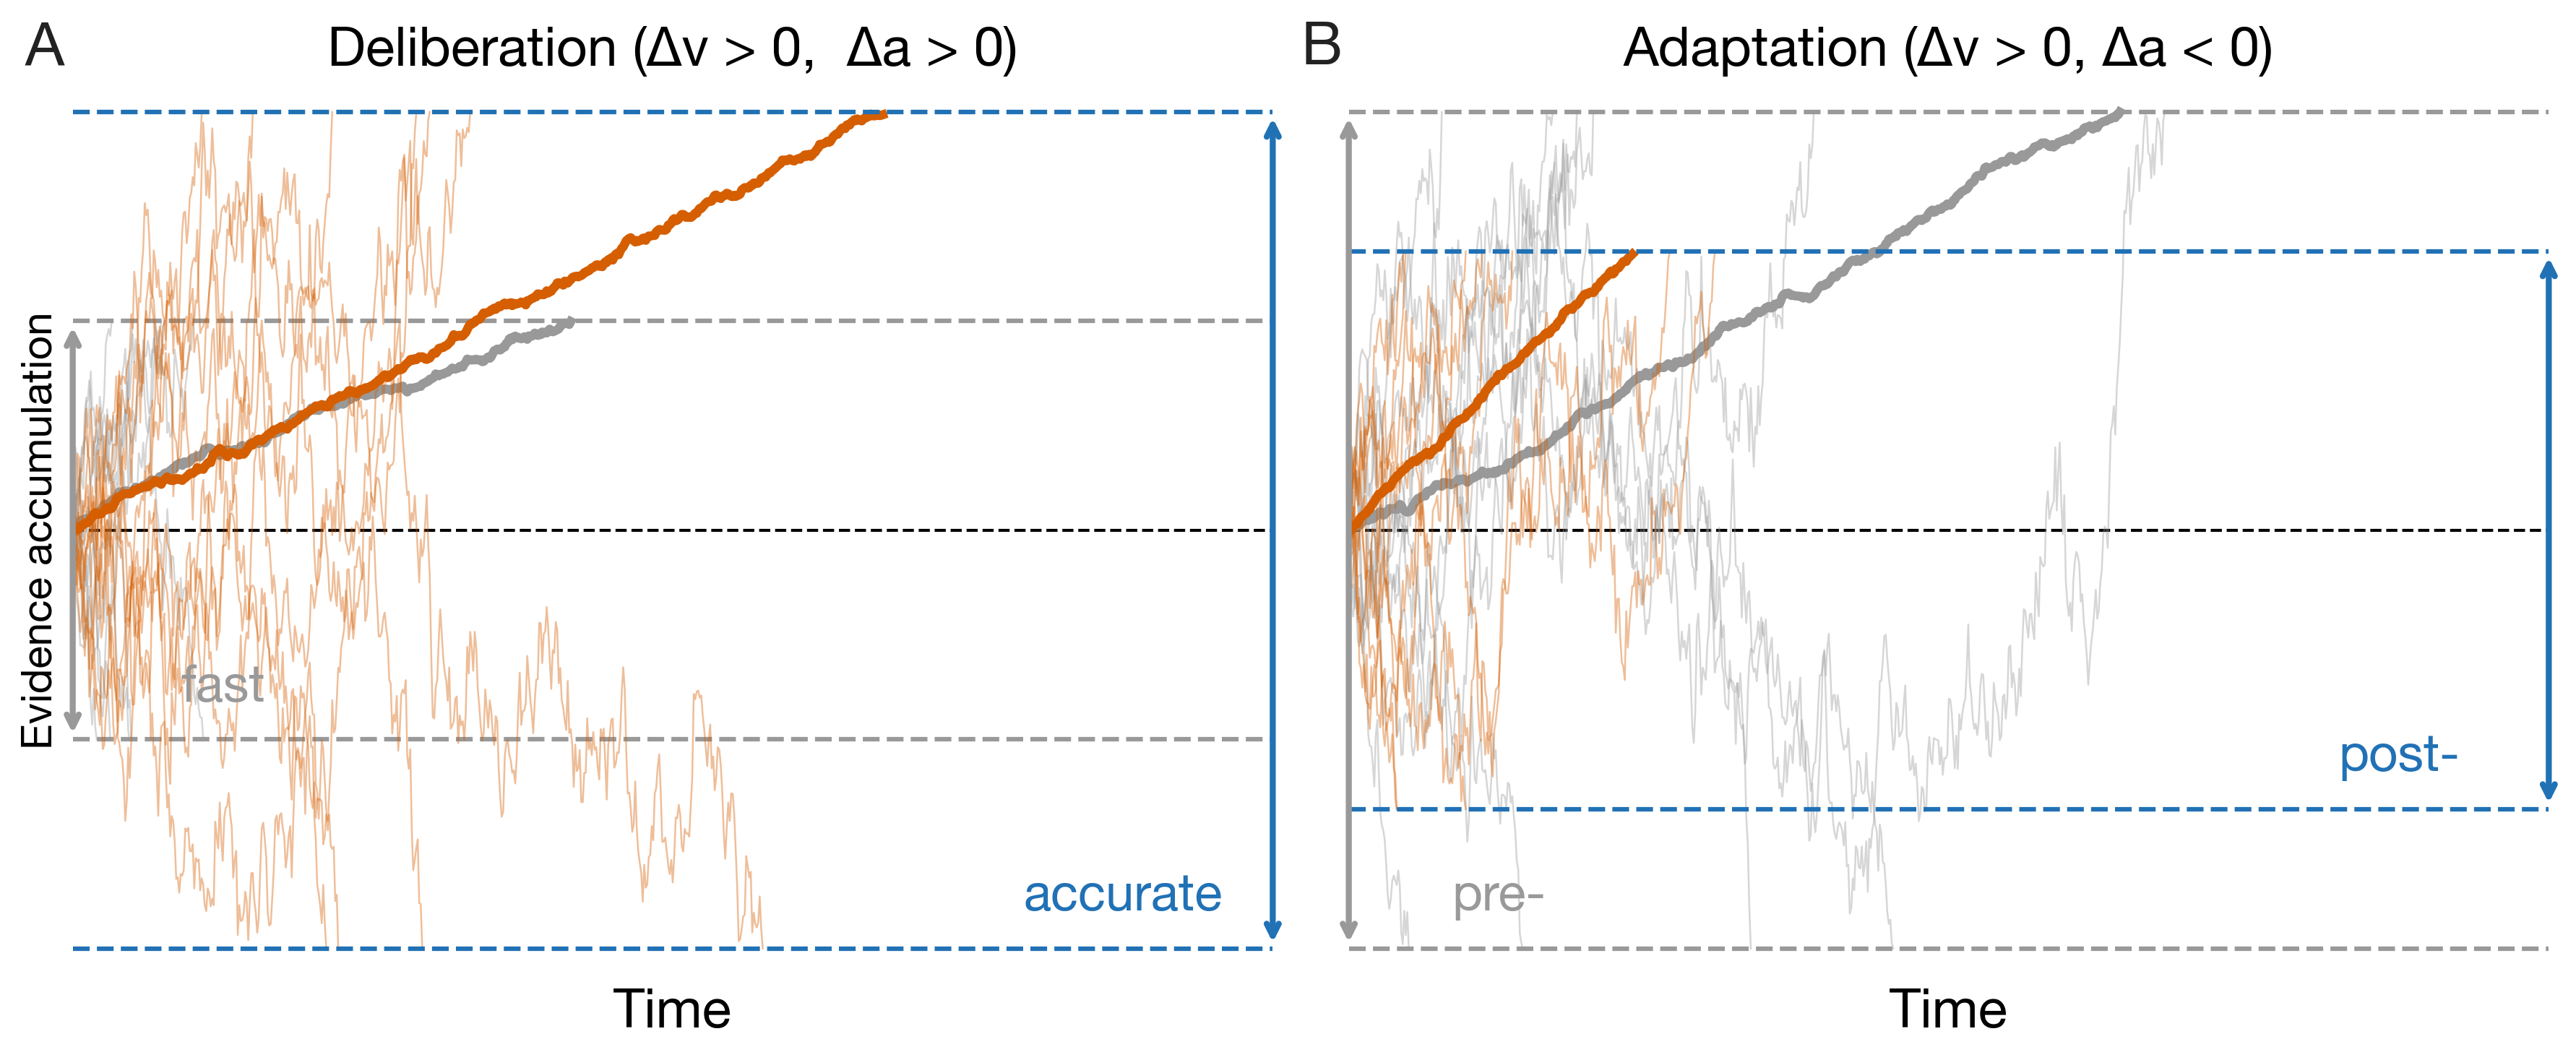
\includegraphics[width=\textwidth]{../figures/Figure1.png}
  \caption{\textbf{Conceptual models of textualism.} (A) In the deliberation model, a reflective mindset elevates the evidence threshold, $\Delta a > 0$, which in turn fosters textualist rule enforcement by increasing net drift toward the textualist response, $\Delta v > 0$. (B) In the adaptation model, net drift toward the textualist response increases, $\Delta v > 0$, and the evidence threshold lowers, $\Delta a < 0$, with greater task experience.}
  \label{fig:conceptual}
\end{figure}

We evaluated the predictions of the deliberation and adaptation accounts by modeling decisions and reaction times through the drift diffusion framework\cite{ref14,ref15}. The core insight of the drift diffusion model (DDM) is that decision-making is a stochastic process of evidence accumulation defined by a threshold and a drift rate. The threshold, $a$, represents the amount of evidence the decision-maker requires before making a decision, which can be understood as the degree of response caution. When a decision is perceived as requiring more evidence (e.g., picking a college major vs.\ an afternoon snack), $a$ adopts a larger value. The drift rate, $v$, captures the average speed at which evidence toward the decision accumulates. Thus, decision time is proportional to the threshold divided by the drift rate, $a/v$. Applications of this framework to interference tasks, such as Stroop and Flanker, have shown that drift rates are faster in congruent trials than in incongruent trials. When both decision boundaries are equidistant from the starting point of evidence accumulation, bias is absent ($z = .50$). Alternatively, when the starting point of evidence accumulation is closer to one decision boundary than the other ($z \neq .50$) decision-making can be described as biased. Finally, total reaction time is composed of both decision time and non-decision time, $t$, i.e., the time employed in parsing the relevant stimuli before the decision process initiates (e.g., reading), plus executing the requisite motor response (e.g., pressing a button on a keyboard).

The initial objective of our studies was to establish whether an interference effect arises in dilemmas of rule enforcement and whether it stems from slower evidence accumulation, a higher threshold, or both (Studies 1a--c and 2). In follow-up experiments, we tested the predictions of the deliberation and adaptation models in the drift diffusion framework. The deliberation model predicts that inducing response caution (i.e., a higher evidence threshold) elevates net drift and, accordingly, promotes textualist decision-making (see Fig.~\ref{fig:conceptual}a and Studies 3a--b). The adaptation hypothesis predicts that progression through the task yields an increase in net drift, and a collapsing evidence threshold---allowing participants to expend less effort in reaching a decision (see Fig.~\ref{fig:conceptual}b and Studies 4a--b).

%%=============================================================%%
\section{Results}\label{sec:results}
%%=============================================================%%

Participants in Experiments 1a--c ($N = 364$) overwhelmingly recognized that congruent cases of violation violated the rule (94\%), did not comply with the rule (7\%) and deserved punishment (92\%); and the pattern reversed for compliance cases (violated: 4\%; complied: 92\%; punishment: 4\%). Incongruent cases of letter--spirit conflict elicited a textualist response pattern for judgments of violation and compliance: Participants classified literal violations more often as breaking the rule (65\%), and less often as complying with the rule (28\%), than cases of literal compliance (breaking: 28\%, complying: 73\%)\cite{ref3,ref8}. Interestingly, the pattern reversed when assigning punishment---with literal compliance (47\%) slightly more likely to receive punishment than literal violation (41\%). Accordingly, mixed-effects logistic regression models revealed main effects of both text and purpose on violation ($\mathrm{OR}_\text{Text} = 48.23$, $\mathrm{OR}_\text{Purpose} = 8.53$), compliance ($\mathrm{OR}_\text{Text} = 0.02$, $\mathrm{OR}_\text{Purpose} = 0.20$), and punishment ($\mathrm{OR}_\text{Text} = 14.65$, $\mathrm{OR}_\text{Purpose} = 18.92$), all $p$s $< .001$ (see Supplementary Analysis~\hyperref[supp:analysis1]{1}).

Reaction times exhibited effects of text ($\chi^2$s $> 483$, $p$s $<.001$), purpose ($\chi^2$s $> 218$, $p$s $< .001$), and a text$\times$purpose interaction in all three models ($\chi^2$s $> 725$, $p$s $< .001$). The cross-over interactions indicated that participants provided faster responses in congruent cases of violation ($\mathrm{Mdn_{RT}} = 2{,}213$--$2{,}378$~ms) and compliance ($\mathrm{Mdn_{RT}} = 2{,}246$--$2{,}318$~ms) than in incongruent cases violating only the rules' text ($\mathrm{Mdn_{RT}} = 2{,}940$--$3{,}127$~ms) or only their purpose ($\mathrm{Mdn_{RT}} = 2{,}658$--$2{,}906$~ms; see Fig.~\ref{fig:rt_histograms}a). Additionally, we observed effects of responses on reaction times in all three experiments: Judgments that the agent violated the rule were faster than judgments that they did not ($\Delta\mathrm{RT_{Yes-No}} = -260$~ms, $t = -9.04$), and decisions to punish were faster than decisions not to punish ($\Delta\mathrm{RT_{Yes-No}} = -232$~ms, $t = -8.46$), both $p$s $< .001$. The effect reversed for compliance, with shorter reaction times when denying, than when affirming, compliance ($\Delta\mathrm{RT_{Yes-No}} = 245$~ms, $t = 8.71$, $p < .001$)---suggesting that it was not due to acquiescence, but instead to faster conviction than acquittal across dependent measures (see Supplementary Analysis~\hyperref[supp:analysis2]{2}).

\begin{figure}[t]
  \centering
  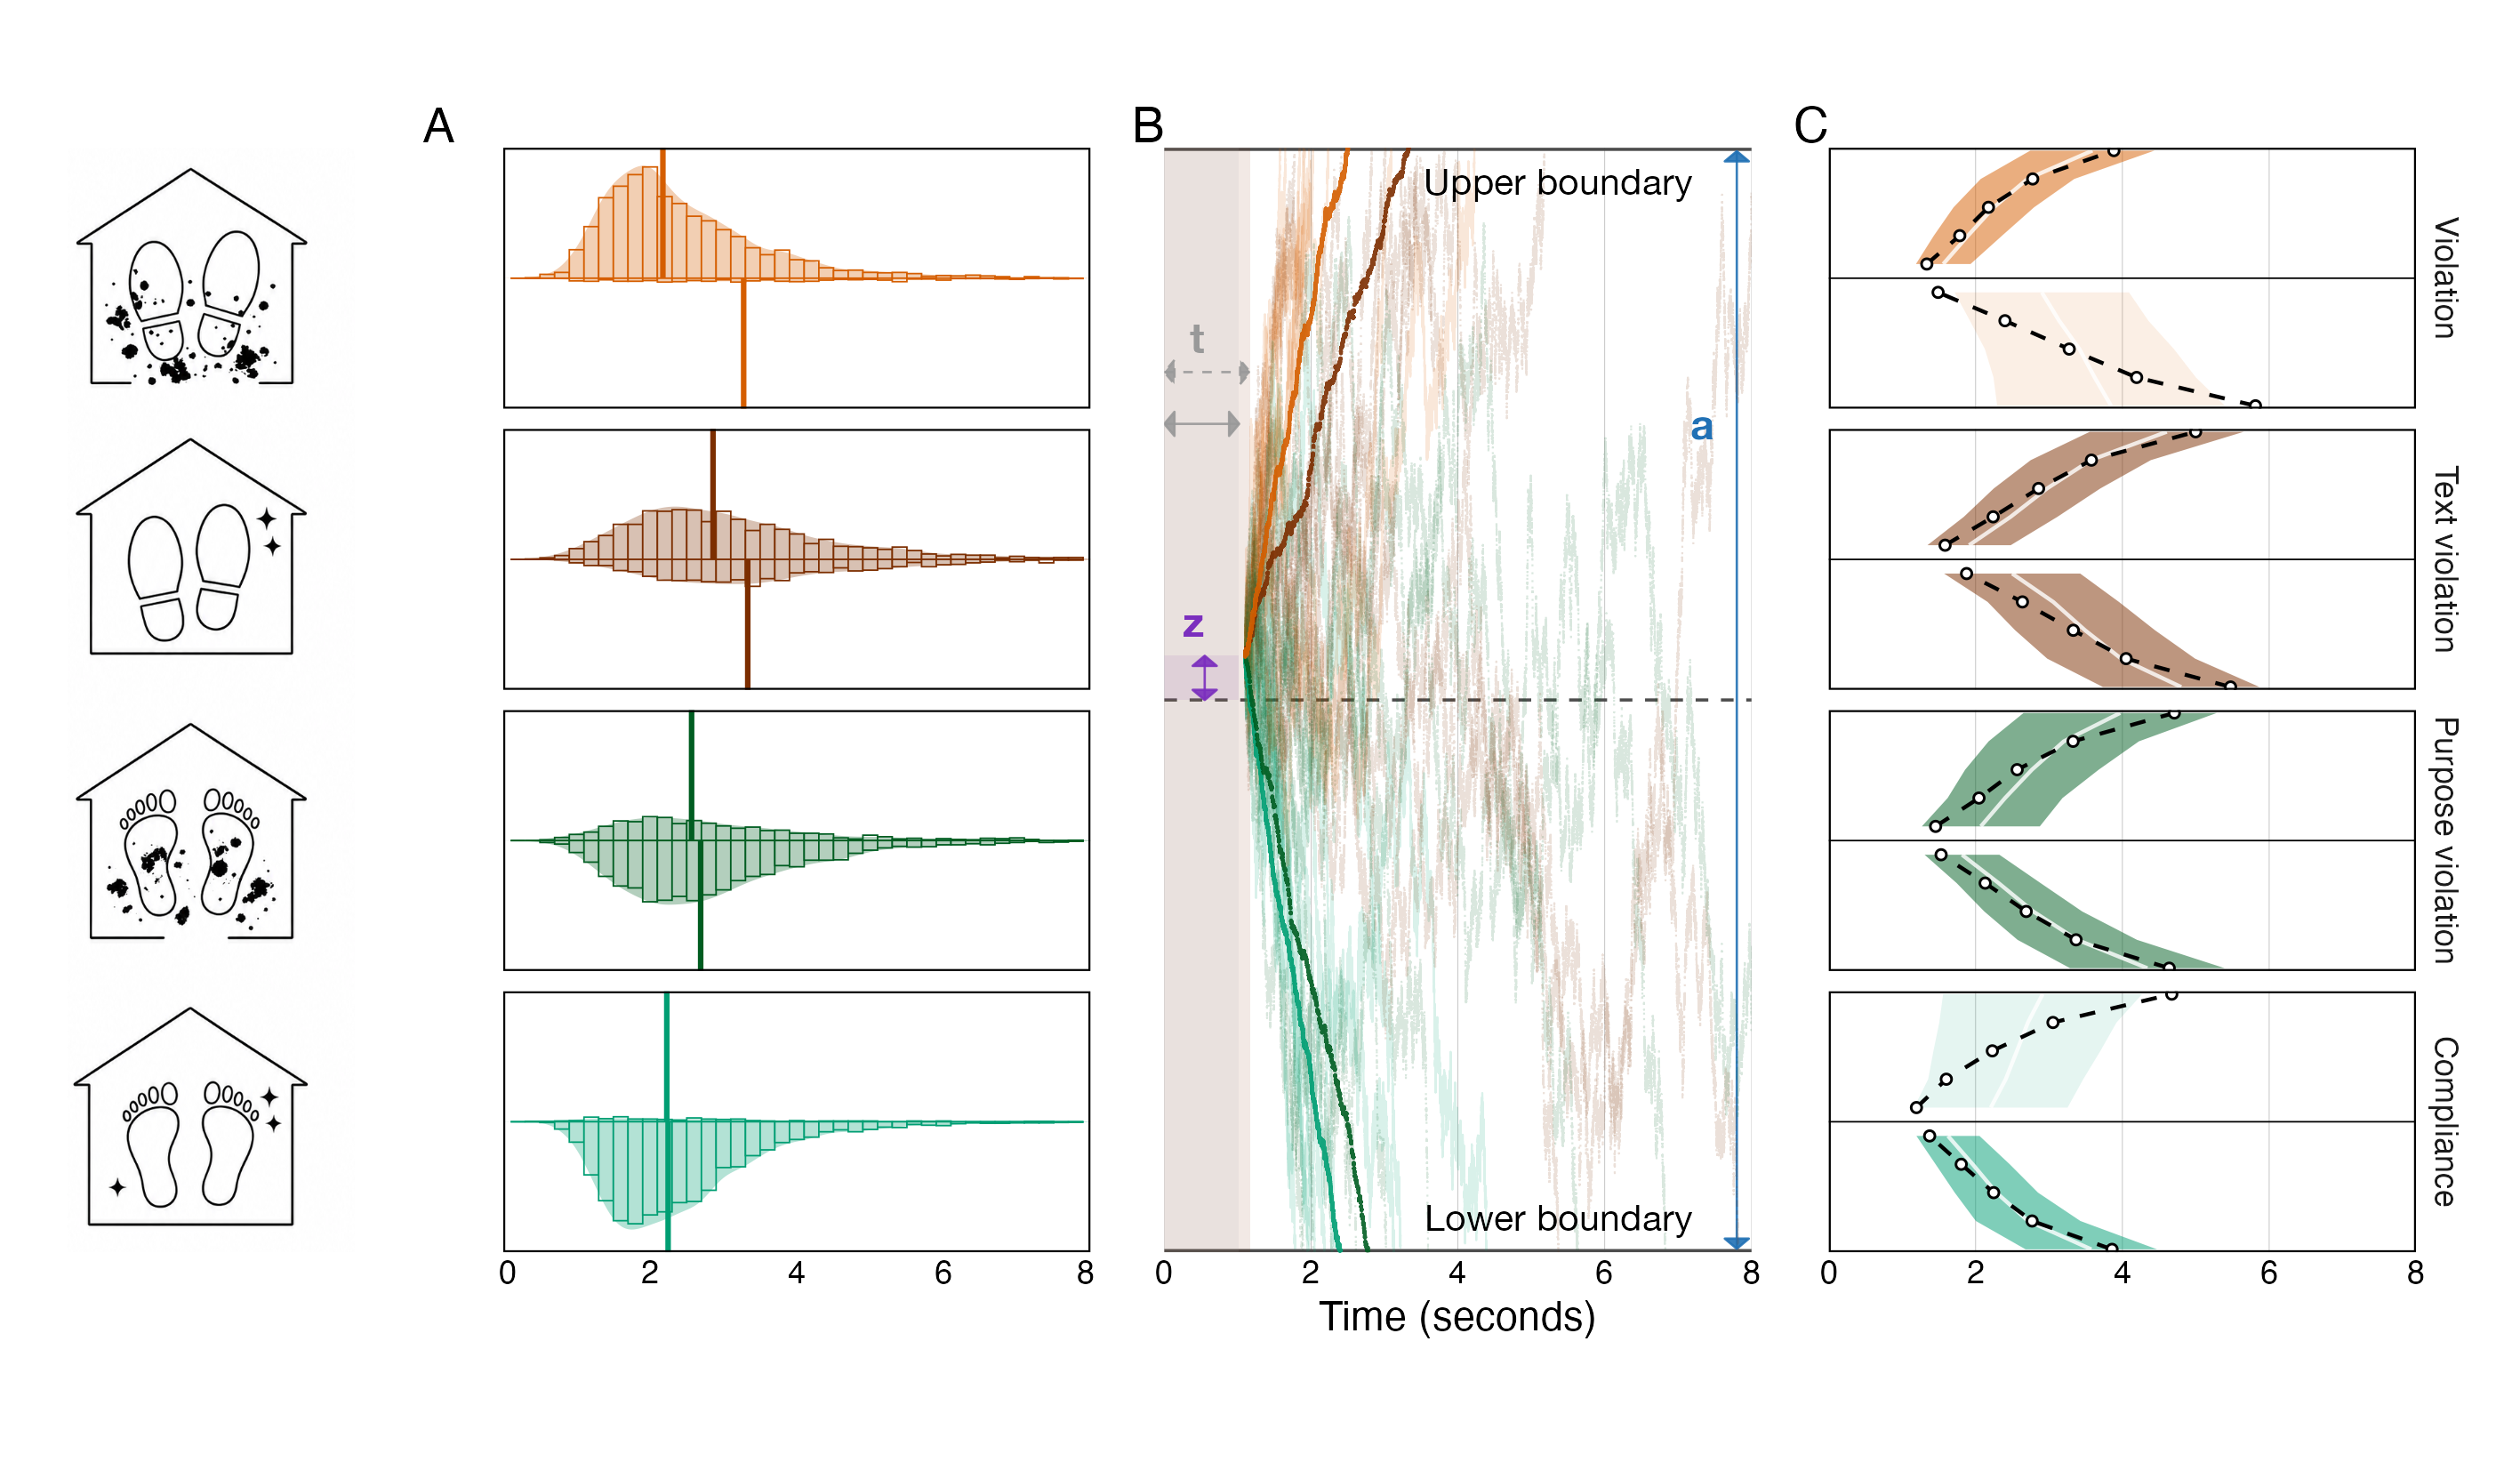
\includegraphics[width=\textwidth]{../figures/Figure2.png}
  \caption{\textbf{Responses, reaction times and the drift diffusion model (DDM) of rule enforcement.} (A) Histograms of reaction times and overlaid medians by response and case-type in Experiment 1a. Upward and downward bars represent `Yes' and `No' responses, respectively. Case-types are displayed in separate rows: violation, literal violation, literal compliance and compliance (from top to bottom). (B) Illustration and (C) posterior predictive checks of the best-fitting hierarchical DDM in Experiment 1a. The illustration highlights the fixed positive bias ($z$) and threshold ($a$), and varying non-decision times ($t$) and drift rates across conditions. The posterior predictive checks show the observed percentiles (10, 30, 50, 70 and 90) for each response and case-type within the 95\% posterior predictive intervals.}
  \label{fig:rt_histograms}
\end{figure}

\subsection{Rule enforcement in the drift diffusion framework}\label{subsec:ddm}

\begin{figure}[b]
  \centering
  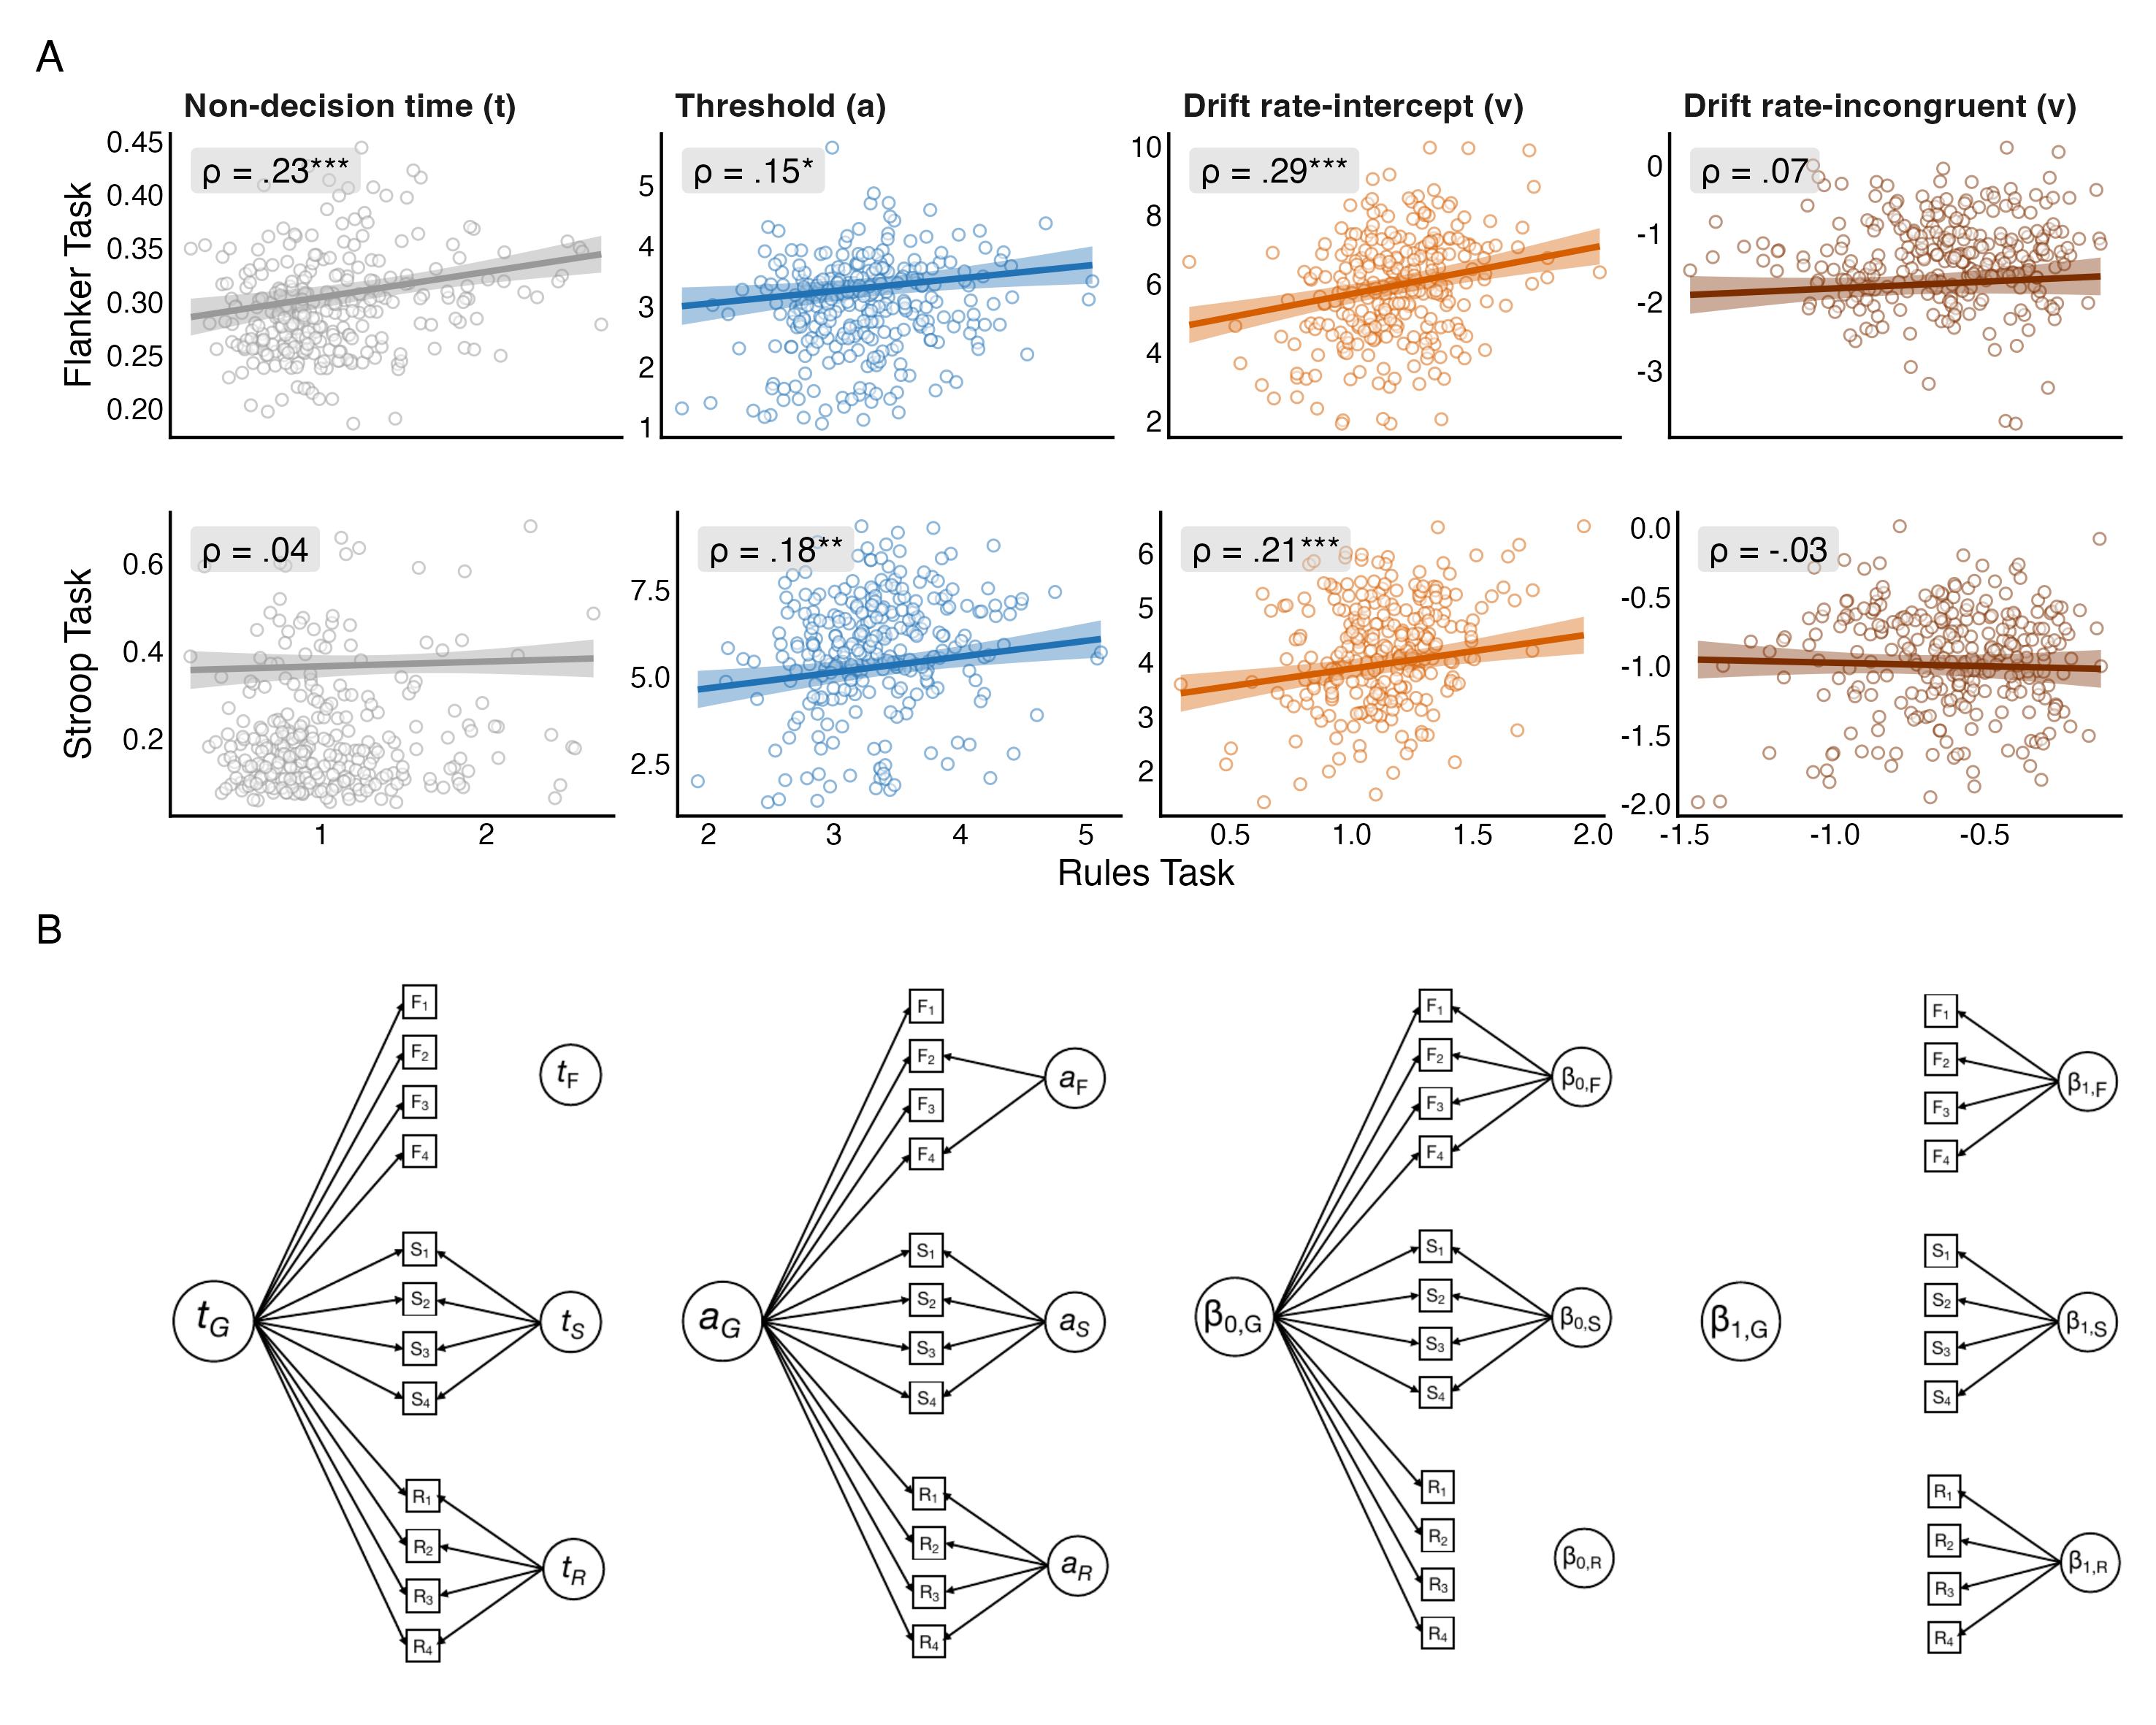
\includegraphics[width=.9\textwidth]{../figures/Figure3.png}
  \caption{\textbf{Cross-task correlations in DDM parameter estimates and bifactor model results.} (A) Scatter plot of drift diffusion parameter estimates from the rule enforcement task ($x$-axis) against corresponding parameters from the interference tasks ($y$-axis). Labels display the Spearman rank correlation coefficients. (B) Results of bifactor models for each decision parameter, displaying general factors on the left (\textit{G} = General) and specific factors on the right (\textit{F} = Flanker, \textit{S} = Stroop, \textit{R} = Rules). Arrows represent significant loadings.}
  \label{fig:cross_task}
\end{figure}

Next, we fit hierarchical drift diffusion models (DDMs) to the reaction time and choice data in the \texttt{hddm} library\cite{ref16}. Posterior predictive checks revealed good fit to the data (see Fig.~\ref{fig:rt_histograms}c and Supplementary Analysis~\hyperref[supp:analysis3]{3}). The best-fitting models indicated that drift rates were substantially faster in congruent cases than incongruent cases (see Fig.~\ref{fig:rt_histograms}b)---both in the comparison between congruent violation ($v = 1.02$, 95\% HDI $[0.94, 1.09]$) and literal violation ($v = 0.23$, 95\% HDI $[0.16, 0.30]$), and between congruent compliance ($v = -1.18$, 95\% HDI $[-1.25, -1.11]$) and literal compliance ($v = -0.52$, 95\% HDI $[-0.59, -0.45]$). This pattern emerged equally when analyzing participants' judgments of compliance and punishment (see Supplementary Analysis~\hyperref[supp:analysis4]{4}). Non-decision times differed modestly across conditions, between 1,014 and 1,161~ms for congruent cases and between 1,119 and 1,371~ms for incongruent cases, contributing partly to longer reaction times in literal violation cases. Participants were biased toward the `yes' response for violation ($z = .54$, 95\% HDI $[.52, .54]$) and punishment ($z = .54$, 95\% HDI $[.53, .55]$), and toward the `no' response ($z = .46$, 95\% HDI $[.45, .47]$) for judgments of compliance---in line with the observed pattern of faster conviction decisions. 

As a further validation of the drift diffusion framework, participants in Experiment 2 ($N = 301$) completed the Stroop and Flanker tasks, along with our rule enforcement task. We fit separate hierarchical DDMs to each task, to understand whether individual estimates in the drift diffusion parameters correlated across tasks. In all three models, threshold and non-decision time were fixed across conditions. To ascertain whether the interference effect on the drift rate correlated across tasks, we specified a coefficient of incongruence, $\beta_1$, controlling for baseline speed of evidence accumulation (on congruent trials), $\beta_0$, such that $v = \beta_0 + \beta_1 \cdot \text{incongruent}$. 

Results indicated that the evidence threshold, the intercept component of the drift rate ($\beta_0$) and, to a lesser extent, non-decision times correlated across tasks (see Fig.~\ref{fig:cross_task}a), pointing to individual differences in these decision parameters. Bifactor models---partitioning variance in each decision parameter into a domain-general factor and domain-specific factors---provided convergent evidence of general factors for non-decision time, threshold, and the baseline drift rate ($\beta_0$, see Fig.~\ref{fig:cross_task}b). Meanwhile, no cross-task associations were found for the incongruence component of the drift rate ($\beta_1$), $|\rho|$s $\leq .07$, $p$s $> .26$, and the bifactor model identified only domain-specific factors for this parameter (see Supplementary Analysis~\hyperref[supp:analysis5]{5}). 

In sum, hierarchical DDMs indicated that the interference effect was primarily attributable to slower evidence accumulation---a signature of cognitive conflict\cite{ref17}---during incongruent cases forcing the choice between applying the rule's letter and its spirit.Thus, individual differences in response caution and overall speed of evidence accumulation correlated across tasks and reflected domain-general decision components. However, the interference effect was uncorrelated across tasks, implying the absence of domain-general, individual differences in inhibitory control. 

\subsection{The deliberation model: Does reflection promote textualist interpretation?}\label{subsec:deliberation}

Having shown that rule enforcement dilemmas elicit cognitive conflict, and validated the use of the drift diffusion framework, we turned to testing the prediction of the deliberation model: i.e., the hypothesis that deliberation, understood as a higher evidence threshold, fosters textualist rule enforcement. 

In Experiment 3a, participants ($N = 123$) applied various rules while instructed to prioritize either decision speed (with a 5-second time limit) or accuracy (with a 10-second time limit) in a counterbalanced order. In previous applications of this paradigm, accuracy instructions have been found to reduce the impact of distractor attributes on responses, thereby improving accuracy\cite{ref18}. Thus, according to the deliberation hypothesis, accuracy instructions should promote response caution and increase net drift---fostering textualist rule interpretation as a result.

Results indicated that accuracy instructions moderated both the effects of text, $\chi^2 = 8.44$, $p = .004$, and purpose, $\chi^2 = 8.31$, $p = .004$. Specifically, accuracy instructions amplified the effects of text ($\mathrm{OR}_{\text{Text}{\cdot}\text{Accuracy}} = 1.46$, $z = 2.91$) and purpose ($\mathrm{OR}_{\text{Purpose}{\cdot}\text{Accuracy}} = 1.45$, $z = 2.88$) relative to speed instructions. Accordingly, accuracy instructions improved classification of congruent cases of violation ($\mathrm{OR}_\text{Accuracy} = 1.33$, $z = 2.32$, $p = .020$) and especially compliance ($\mathrm{OR}_\text{Accuracy} = 0.63$, $z = -3.57$, $p < .001$). Yet, accuracy had no observable effect on judgments of incongruent cases, $p$s $> .26$---owing to suppression between both positive interactions (see Supplementary Analysis~\hyperref[supp:analysis6]{6}).

In Experiment 3b, participants ($N = 121$) were asked to apply rules while we manipulated the proportion of congruent cases in each block (high congruency: 5-to-1, low congruency: 1-to-5). Prior research has shown that changes in the proportion of congruency impact response caution, and accordingly reduce the influence of distractor attributes on responses\cite{ref19}.

Mirroring the results of Experiment 3a, congruency proportion moderated both effects of text, $\chi^2 = 6.44$, $p = .011$, and purpose, $\chi^2 = 5.93$, $p = .014$. Both positive effects of text ($\mathrm{OR}_{\text{Text}{\cdot}\text{Congruency}} = 1.56$, $z = 2.54$) and purpose ($\mathrm{OR}_{\text{Purpose}{\cdot}\text{Congruency}} = 1.53$, $z = 2.44$) were amplified in high congruency blocks, relative to low congruency blocks. As a result, judgments of incongruent cases were unaffected by the proportion of congruency, $p$s $> .072$. Meanwhile, classification of violation cases was more accurate when congruent trials were frequent ($\mathrm{OR}_\text{Congruency} = 1.83$, $z = 3.78$, $p < .001$), whereas the effect on compliance cases was not significant ($\mathrm{OR}_\text{Congruency} = 0.77$, $z = -1.54$, $p = .12$).

Next, we examined the effect of accuracy instructions and congruency proportion on the four decision parameters in hierarchical DDM regressions (see model specification in Table~\ref{tab:hddm}).

\begin{table}[h]
\caption{HDDM regression models in Experiments 3a and 3b.}
\label{tab:hddm}
\begin{tabular}{@{}llp{9cm}@{}}
\toprule
Parameter & Exp. & Specification \\
\midrule
\multirow{2}{*}{Drift rate} & 3a & 
$v = \beta_{0,v} + \beta_{1,v}{\cdot}\text{text} + \beta_{2,v}{\cdot}\text{purpose} + \beta_{3,v}{\cdot}\text{acc.} + \beta_{4,v}{\cdot}\text{text}{\cdot}\text{acc.} + \beta_{5,v}{\cdot}\text{purpose}{\times}\text{acc.}
$ \\
                            & 3b & 
                            $v = \beta_{0,v} + \beta_{1,v}{\cdot}\text{text} + \beta_{2,v}{\cdot}\text{purpose} + \beta_{3,v}{\cdot}\text{prop.} + \beta_{4,v}{\cdot}\text{text}{\cdot}\text{prop.} + \beta_{5,v}{\cdot}\text{purpose}{\times}\text{prop.}
                            $ \\
\multirow{2}{*}{Threshold} & 3a & $a = \beta_{0,a} + \beta_{1,a}{\cdot}\text{acc.}$ \\
                                & 3b & $a = \beta_{0,a} + \beta_{1,a}{\cdot}\text{prop.}$ \\
\multirow{2}{*}{Non-decision time} & 3a & $t = \beta_{0,t} + \beta_{1,t}{\cdot}\text{acc.} + \beta_{2,t}{\cdot}\text{inc.} + \beta_{3,t}{\cdot}\text{acc.}{\cdot}\text{inc.}$ \\
                                    & 3b & $t = \beta_{0,t} + \beta_{1,t}{\cdot}\text{prop.} + \beta_{2,t}{\cdot}\text{inc.} + \beta_{3,t}{\cdot}\text{prop.}{\cdot}\text{inc.}$ \\
\multirow{2}{*}{Bias} & 3a & $z = \beta_{0,z} + \beta_{1,z}{\cdot}\text{acc.}$ \\
                       & 3b & $z = \beta_{0,z} + \beta_{1,z}{\cdot}\text{prop.}$ \\
\bottomrule
\end{tabular}
\footnotetext{acc.\ = accuracy condition, inc.\ = incongruent trial, prop.\ = congruency proportion.}
\end{table}

Both manipulations successfully induced response caution: Participants employed a higher evidence threshold under accuracy instructions (vs. speed: $\beta_{1,a} = 0.65$, 95\% HDI $[0.53, 0.76]$), and in high congruency blocks (vs. low: $\beta_{1,a} = 0.49$, 95\% HDI $[0.34, 0.63]$). However, neither manipulation produced net textualist drift: Instructions to prioritize accuracy over speed attenuated the text component ($\beta_{4,v} = -0.17$, 95\% HDI $[-0.26, -0.08]$) without affecting the purpose component ($\beta_{5,v} = 0.00$, 95\% HDI $[-0.08, 0.08]$), of the drift rate. Meanwhile, high congruency blocks strengthened both drift components of text ($\beta_{4,v} = 0.23$, 95\% HDI $[0.13, 0.33]$) and purpose equally ($\beta_{5,v} = 0.27$, 95\% HDI $[0.20, 0.35]$). 

Accuracy instructions increased non-decision time ($\beta_{1,t} = 0.08$, 95\% HDI $[0.02, 0.15]$). The proportion manipulation also influenced non-decision times, which were generally shorter in high congruency blocks (vs. low congruency blocks; $\beta_{1,t} = -0.22$, 95\% HDI $[-0.27, -0.16]$). Lastly, bias did not differ across conditions in either experiment (see Supplementary Analysis~\hyperref[supp:analysis8]{8}).

Experiments 3a and 3b manipulated the time limit within which to make a decision (i.e., keeping work constant and adding time) and the blockwise proportion of congruent trials (i.e., keeping time constant and adding work). These manipulations influenced response caution: Participants elevated the evidence threshold when given either extra time to solve the same cases (i.e., under accuracy instructions), or effectively less cognitive work to do in the same time frame (i.e., with fewer incongruent cases per block). Contrary to the deliberation hypothesis, however, greater response caution did not produce a shift toward textualist rule enforcement in either experiment.

\subsection{The adaptation model: Does textualism develop with experience?}\label{subsec:adaptation}

Multiple strands of research have documented resource-rational adaptations to cognitively demanding tasks\cite{ref20,ref21,ref22}. Generally, these adaptations aim to reduce cognitive effort while preserving accuracy---i.e., to optimize the effort-accuracy trade-off. A re-analysis of Experiments 1a--3b revealed that participants issued quicker decisions by the end of the experiments ($\Delta\mathrm{RT_{Trial}} = -544$~ms, $t = -54.19$, $p < .001$) and gravitated toward textualist enforcement---as revealed by a trial proportion$\cdot$text interaction ($\mathrm{OR}= 1.78$, 95\% CI $[1.52, 2.09]$, $z = 7.08$, $p < .001$, see Supplementary Analysis~\hyperref[supp:analysis9]{9}). As shown in Figure~\ref{fig:exp4a}a, this effect translated into greater conviction of literal violations ($\mathrm{OR}= 1.39$, 95\% CI $[1.25, 1.53]$, $z = 6.31$), and greater acquittal of literal compliance ($\mathrm{OR}= 0.71$, 95\% CI $[0.63, 0.79]$, $z = -6.27$), $ps < .001$.

\begin{figure}[b]
  \centering
  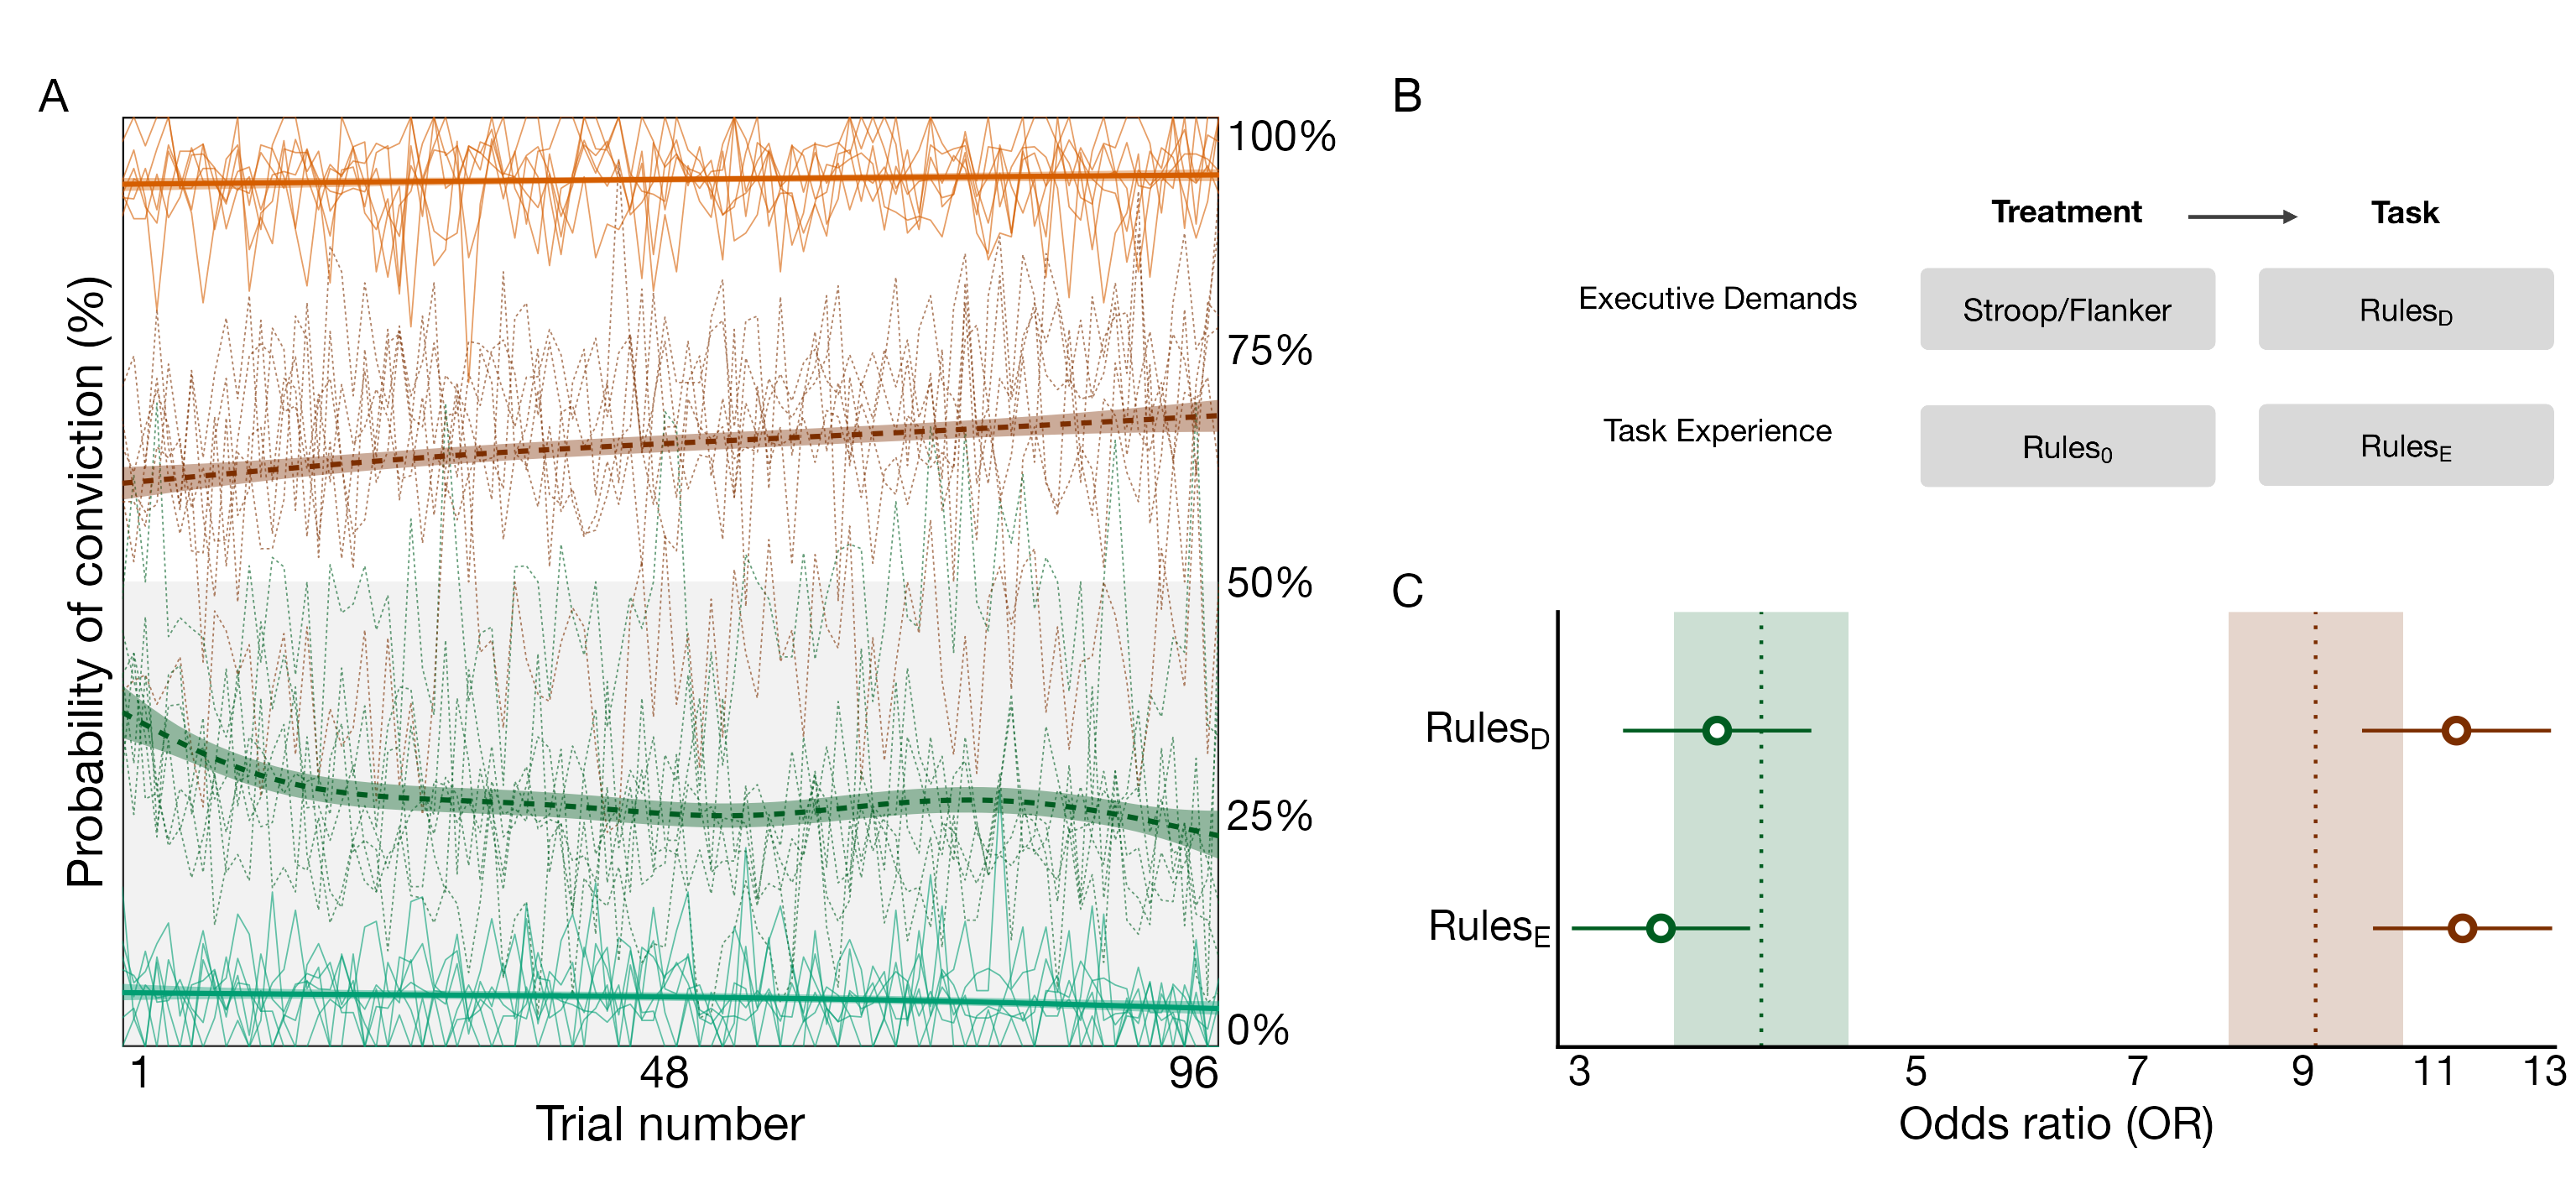
\includegraphics[width=\textwidth]{../figures/Figure4.png}
  \caption{\textbf{Effects of trial number, task experience and executive demands.} (A) Probability of a conviction decision by trial number and case-type in a mega-analysis of Studies 1a-3b (\textit{N} = 909, \textit{n} = 85,819). Solid lines represent congruent cases and dashed lines represent incongruent cases. Colors distinguish text violation from compliance cases. (B) Schematic diagram and (C) results of Experiment 4a. Regression coefficients of text and purpose by treatment on the log-odds scale. Dotted lines and confidence bands display the corresponding coefficients in the baseline block, Rules$_0$. Both the Task Experience and Executive Demand treatments strengthened the effect of text.}
  \label{fig:exp4a}
\end{figure}

We designed two final experiments to replicate and extend this exploratory finding, asking whether textual interpretation develops specifically through learning, i.e., from experience with rule enforcement, or more generally from executive demands.

Participants ($N = 227$) in Experiment 4a took part in four blocks of the Rules task and we manipulated whether they previously completed four baseline blocks of the same Rules task (Task Experience condition), or four blocks of Stroop and Flanker tasks in a randomized order (Executive Demand condition; see Fig.~\ref{fig:exp4a}b). The learning hypothesis predicts elevated textualism as a result of task experience only, whereas the effort hypothesis predicts elevated textualism whether in response to specific task experience or to exogenous cognitive demands.

As in the exploratory analysis, the effect of text strengthened over the course of the experiment, $\mathrm{OR}_{\text{Trial}{\cdot}\text{Text}} = 1.65$, 95\% CI $[1.19, 2.29]$, $z = 2.97$, $p = .003$, and the effect of purpose weakened, $\mathrm{OR}_{\text{Trial}{\cdot}\text{Purpose}} = 0.69$, 95\% CI $[0.49, 0.95]$, $z = -2.24$, $p = .025$. At the block level, both Task Experience ($\mathrm{OR}_{\text{Block}{\cdot}\text{Text}} = 1.25$, 95\% CI $[1.03, 1.51]$, $z = 2.31$, $p = .021$) and Executive Demand ($\mathrm{OR}_{\text{Block}{\cdot}\text{Text}} = 1.24$, 95\% CI $[1.02, 1.51]$, $z = 2.15$, $p = .032$) treatments strengthened the effect of text. By contrast, the effect of purpose did not differ across blocks ($\mathrm{OR}_{\text{Block}{\cdot}\text{Purpose}} = 0.86$, $z = -1.58$, $p = .11$; $\mathrm{OR}_{\text{Block}{\cdot}\text{Purpose}} = 0.94$, $z = -0.68$, $p = .50$; see Fig.~\ref{fig:exp4a}c and Supplementary Analysis~\hyperref[supp:analysis10]{10}). Thus, results supported the effort hypothesis, showing that participants' spontaneous shift toward textualism occurred in reaction to executive demands, whether from rule enforcement or unrelated interference tasks. 

In Experiment 4b, we confirmed this pattern by assessing pre-to-post change across three between-subjects treatments: the Executive Demand (4 blocks of Stroop and Flanker interference tasks) and Task Experience (4 additional blocks of the Rules task) treatments, as well as a Passive Control condition (viewing a 3-minute time lapse video). Participants ($N = 600$) completed a pre-treatment block of the Rules task, followed by the randomly assigned treatment, and a post-treatment block of the Rules task.

The shift toward textual enforcement manifested in two ways (see Fig.~\ref{fig:exp4b}a): as a reduced influence of purpose after the Executive Demand, $\mathrm{OR}_{\text{Block}{\cdot}\text{Purpose}} = 0.64$, $z = -3.56$, $p < .001$, and Task Experience treatments, $\mathrm{OR}_{\text{Block}{\cdot}\text{Purpose}} = 0.61$, $z = -3.65$, $p < .001$ (but Passive Control: $\mathrm{OR}_{\text{Block}{\cdot}\text{Purpose}} = 0.88$, $z = -0.95$, $p = .34$) and as an increased effect of text after the Executive Demand treatment, $\mathrm{OR}_{\text{Block}{\cdot}\text{Text}} = 1.33$, $z = 2.39$, $p = .017$ (Task Experience: $\mathrm{OR}_{\text{Block}{\cdot}\text{Text}} = 0.90$, $z = -0.45$, $p = .65$; Passive Control: $\mathrm{OR}_{\text{Block}{\cdot}\text{Text}} = 1.27$, $z = 1.85$, $p = .065$).

\begin{figure}[t]
  \centering
  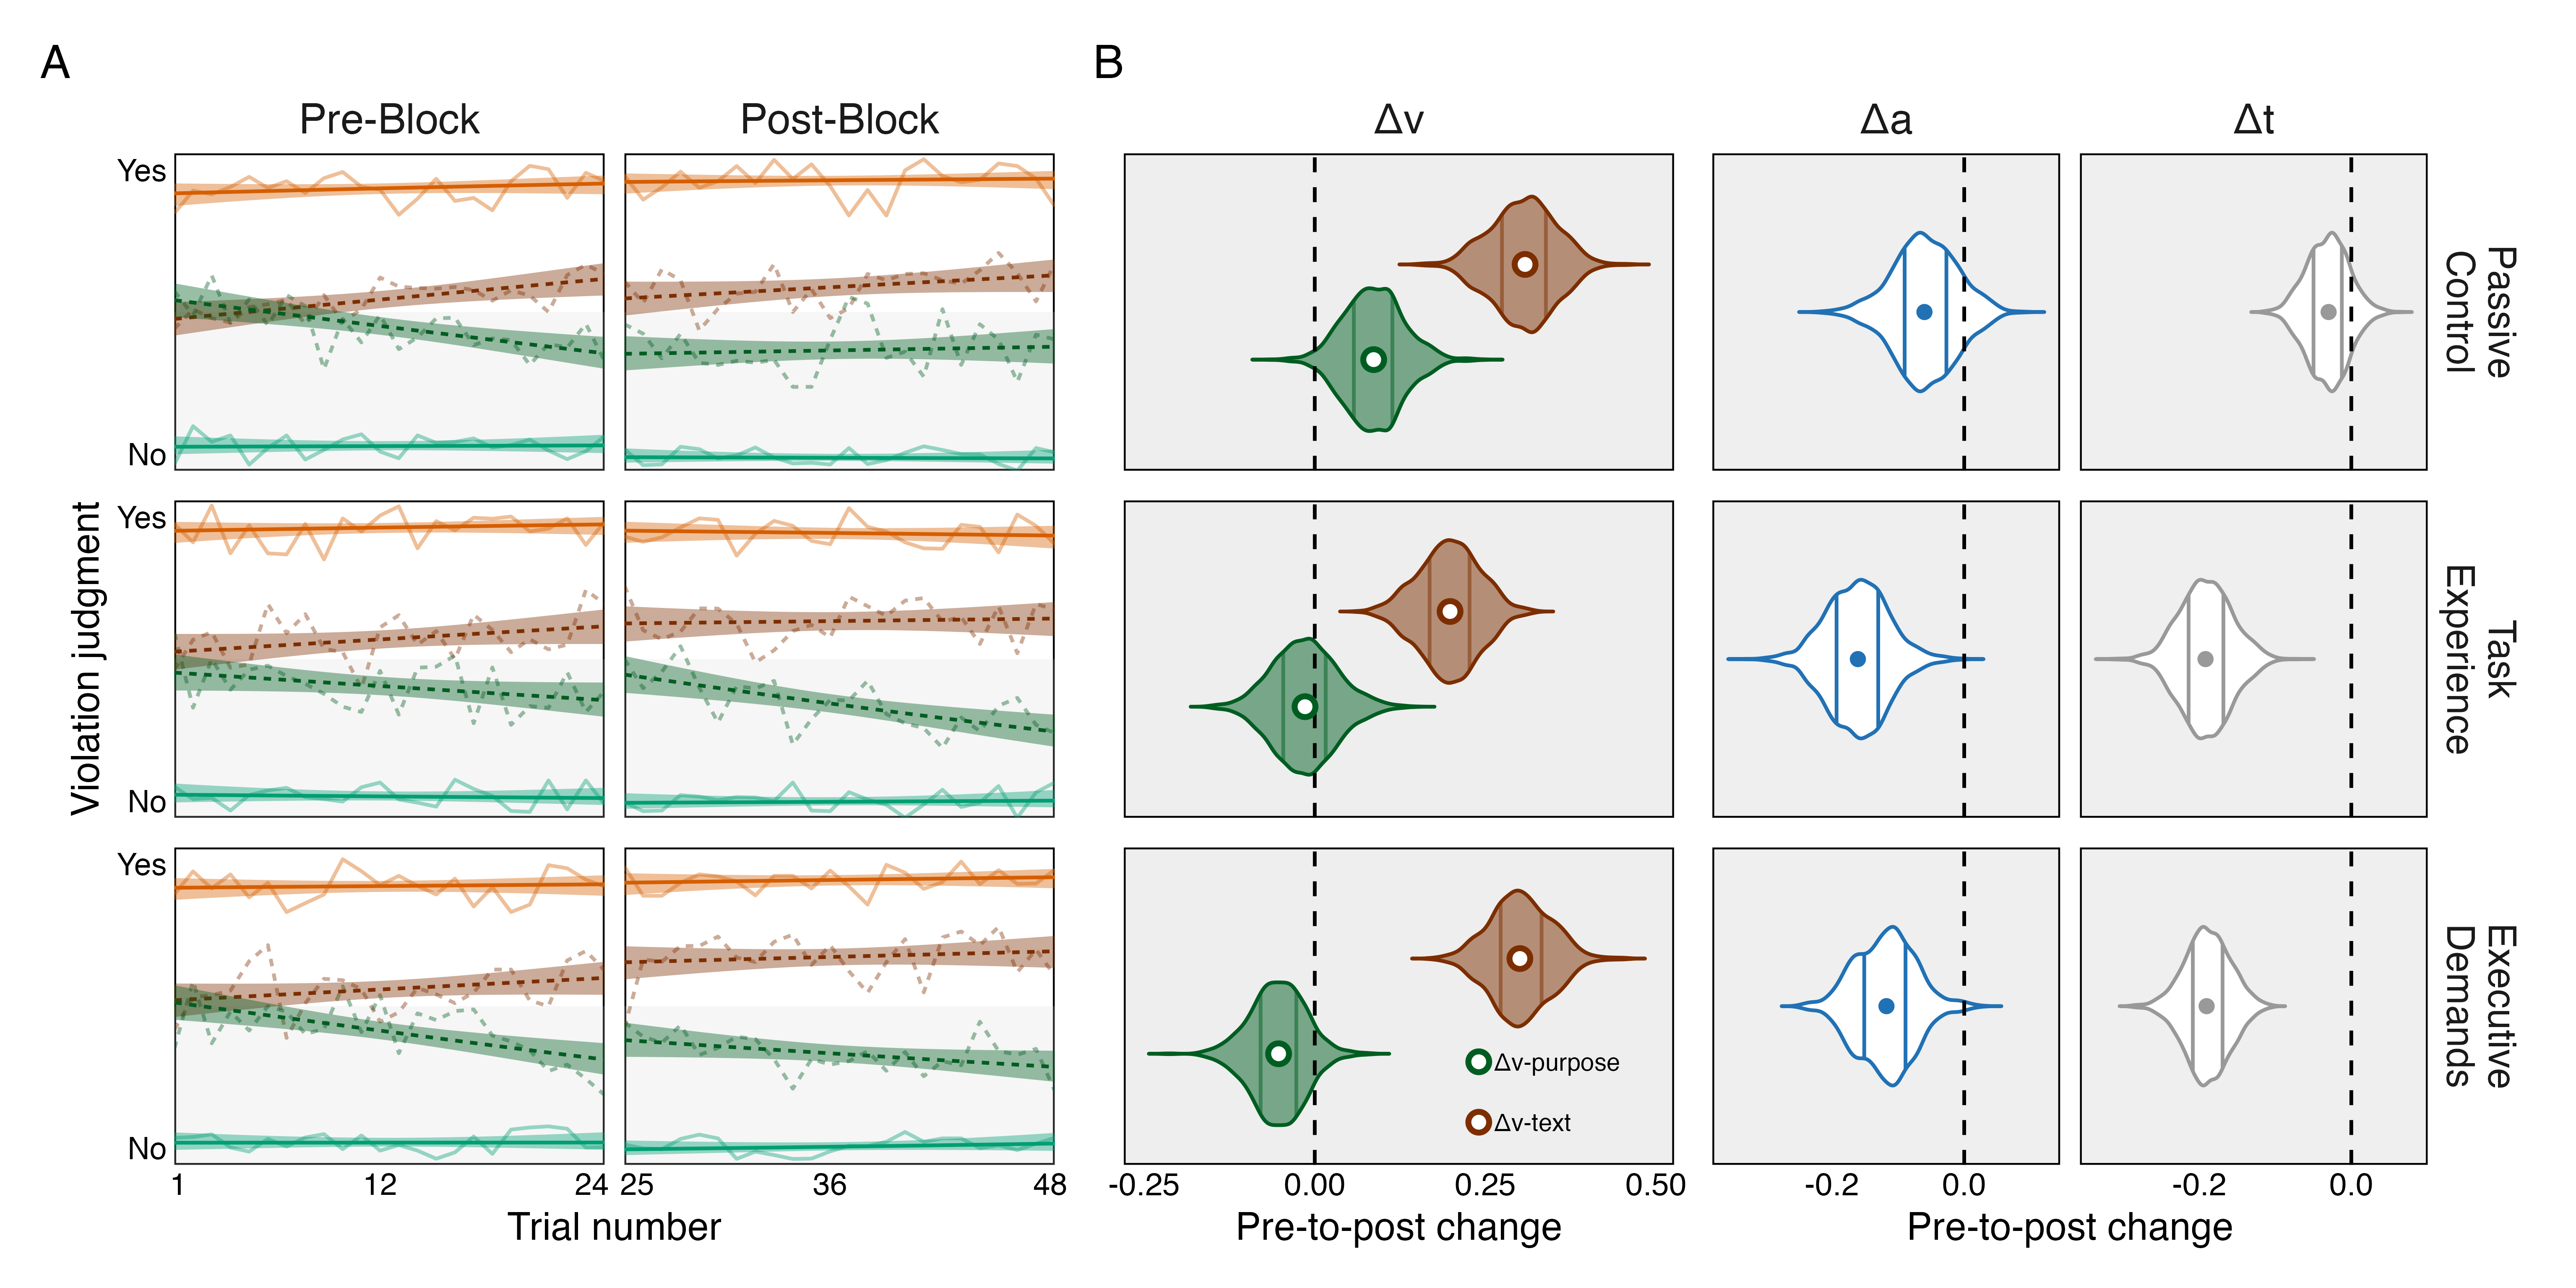
\includegraphics[width=\textwidth]{../figures/Figure5.png}
  \caption{\textbf{Results of Experiment 4b.} (A) Effect of trial number on the probability of a violation decision by case-type and treatment condition. Solid lines represent congruent cases and dashed lines represent incongruent cases. Colors distinguish text violation from compliance cases. (B) Posterior distributions of the HDDM parameter change scores by treatment condition. Vertical lines represent the interquartile range, and overlaid dots display the posterior means.}
  \label{fig:exp4b}
\end{figure}

Hierarchical DDMs revealed underlying changes in the decision parameters in both experiments. In Experiment 4a, task experience lowered the evidence threshold ($a_\text{Block} = -0.21$, 95\% HDI $[-0.27, -0.15]$) and shortened non-decision times ($t_\text{Block} = -0.04$, 95\% HDI $[-0.06, -0.01]$), whereas executive demands had no credible effects ($a_\text{Block} = -0.11$, 95\% HDI $[-0.26, 0.06]$; $t_\text{Block} = -0.06$, 95\% HDI $[-0.15, 0.01]$). In Experiment 4b, when assessed against a within-subjects baseline, both task experience and domain-general cognitive demands reduced the evidence threshold (Executive Demand: $\Delta a = -0.12$, 95\% HDI $[-0.20, -0.03]$; Task Experience: $\Delta a = -0.16$, 95\% HDI $[-0.25, -0.07]$) and non-decision time (Executive Demand: $\Delta t = -0.19$, 95\% HDI $[-0.25, -0.13]$; Task Experience: $\Delta t = -0.19$, 95\% HDI $[-0.26, -0.12]$). Thus, both task experience and executive demands lowered the evidence threshold, when compared to pre-treatment blocks. This pattern is consistent with a strategic reduction in effort, as participants were able to make faster decisions by lowering the amount of evidence required to reach a decision. 

Task experience and executive demands also produced a change toward faster accumulation of textualist evidence, but not purposive evidence. In Experiment 4a, the drift component of text increased through both task experience ($v_{\text{Block}{\cdot}\text{Text}} = 0.14$, 95\% HDI $[0.08, 0.21]$) and domain-general executive demand ($v_{\text{Block}{\cdot}\text{Text}} = 0.11$, 95\% HDI $[0.04, 0.17]$) relative to the baseline block, Rules$_0$. These effects replicated in Experiment 4b, with credible pre-to-post increases in the drift component of text (Executive Demand: $\Delta v_\text{Text} = 0.30$, 95\% HDI $[0.22, 0.39]$; Task Experience: $\Delta v_\text{Text} = 0.20$, 95\% HDI $[0.11, 0.28]$). No corresponding effects emerged with the drift component of purpose in either experiment (4a: Rules$_E$: $v_{\text{Block}{\cdot}\text{Purpose}} = -0.03$, 95\% HDI $[-0.09, 0.04]$; Rules$_D$: $v_{\text{Block}{\cdot}\text{Purpose}} = -0.01$, 95\% HDI $[-0.07, 0.05]$; 4b: Executive Demand: $\Delta v_\text{Purpose} = -0.05$, 95\% HDI $[-0.14, 0.02]$; Task Experience: $\Delta v_\text{Purpose} = -0.01$, 95\% HDI $[-0.10, 0.08]$). 

The passive control treatment, with minimal executive demands, yielded increases in \textit{both} drift components of text ($\Delta v_\text{Text} = 0.31$, 95\% HDI $[0.22, 0.39]$) and purpose ($\Delta v_\text{Purpose} = 0.09$, 95\% HDI $[0.01, 0.17]$), and produced no credible change in the evidence threshold ($\Delta a = -0.06$, 95\% HDI $[-0.16, 0.03]$) or non-decision time ($\Delta t = -0.03$, 95\% HDI $[-0.08, 0.02]$; see Supplementary Analysis~\hyperref[supp:analysis11]{11}).

\begin{figure}[t]
  \centering
  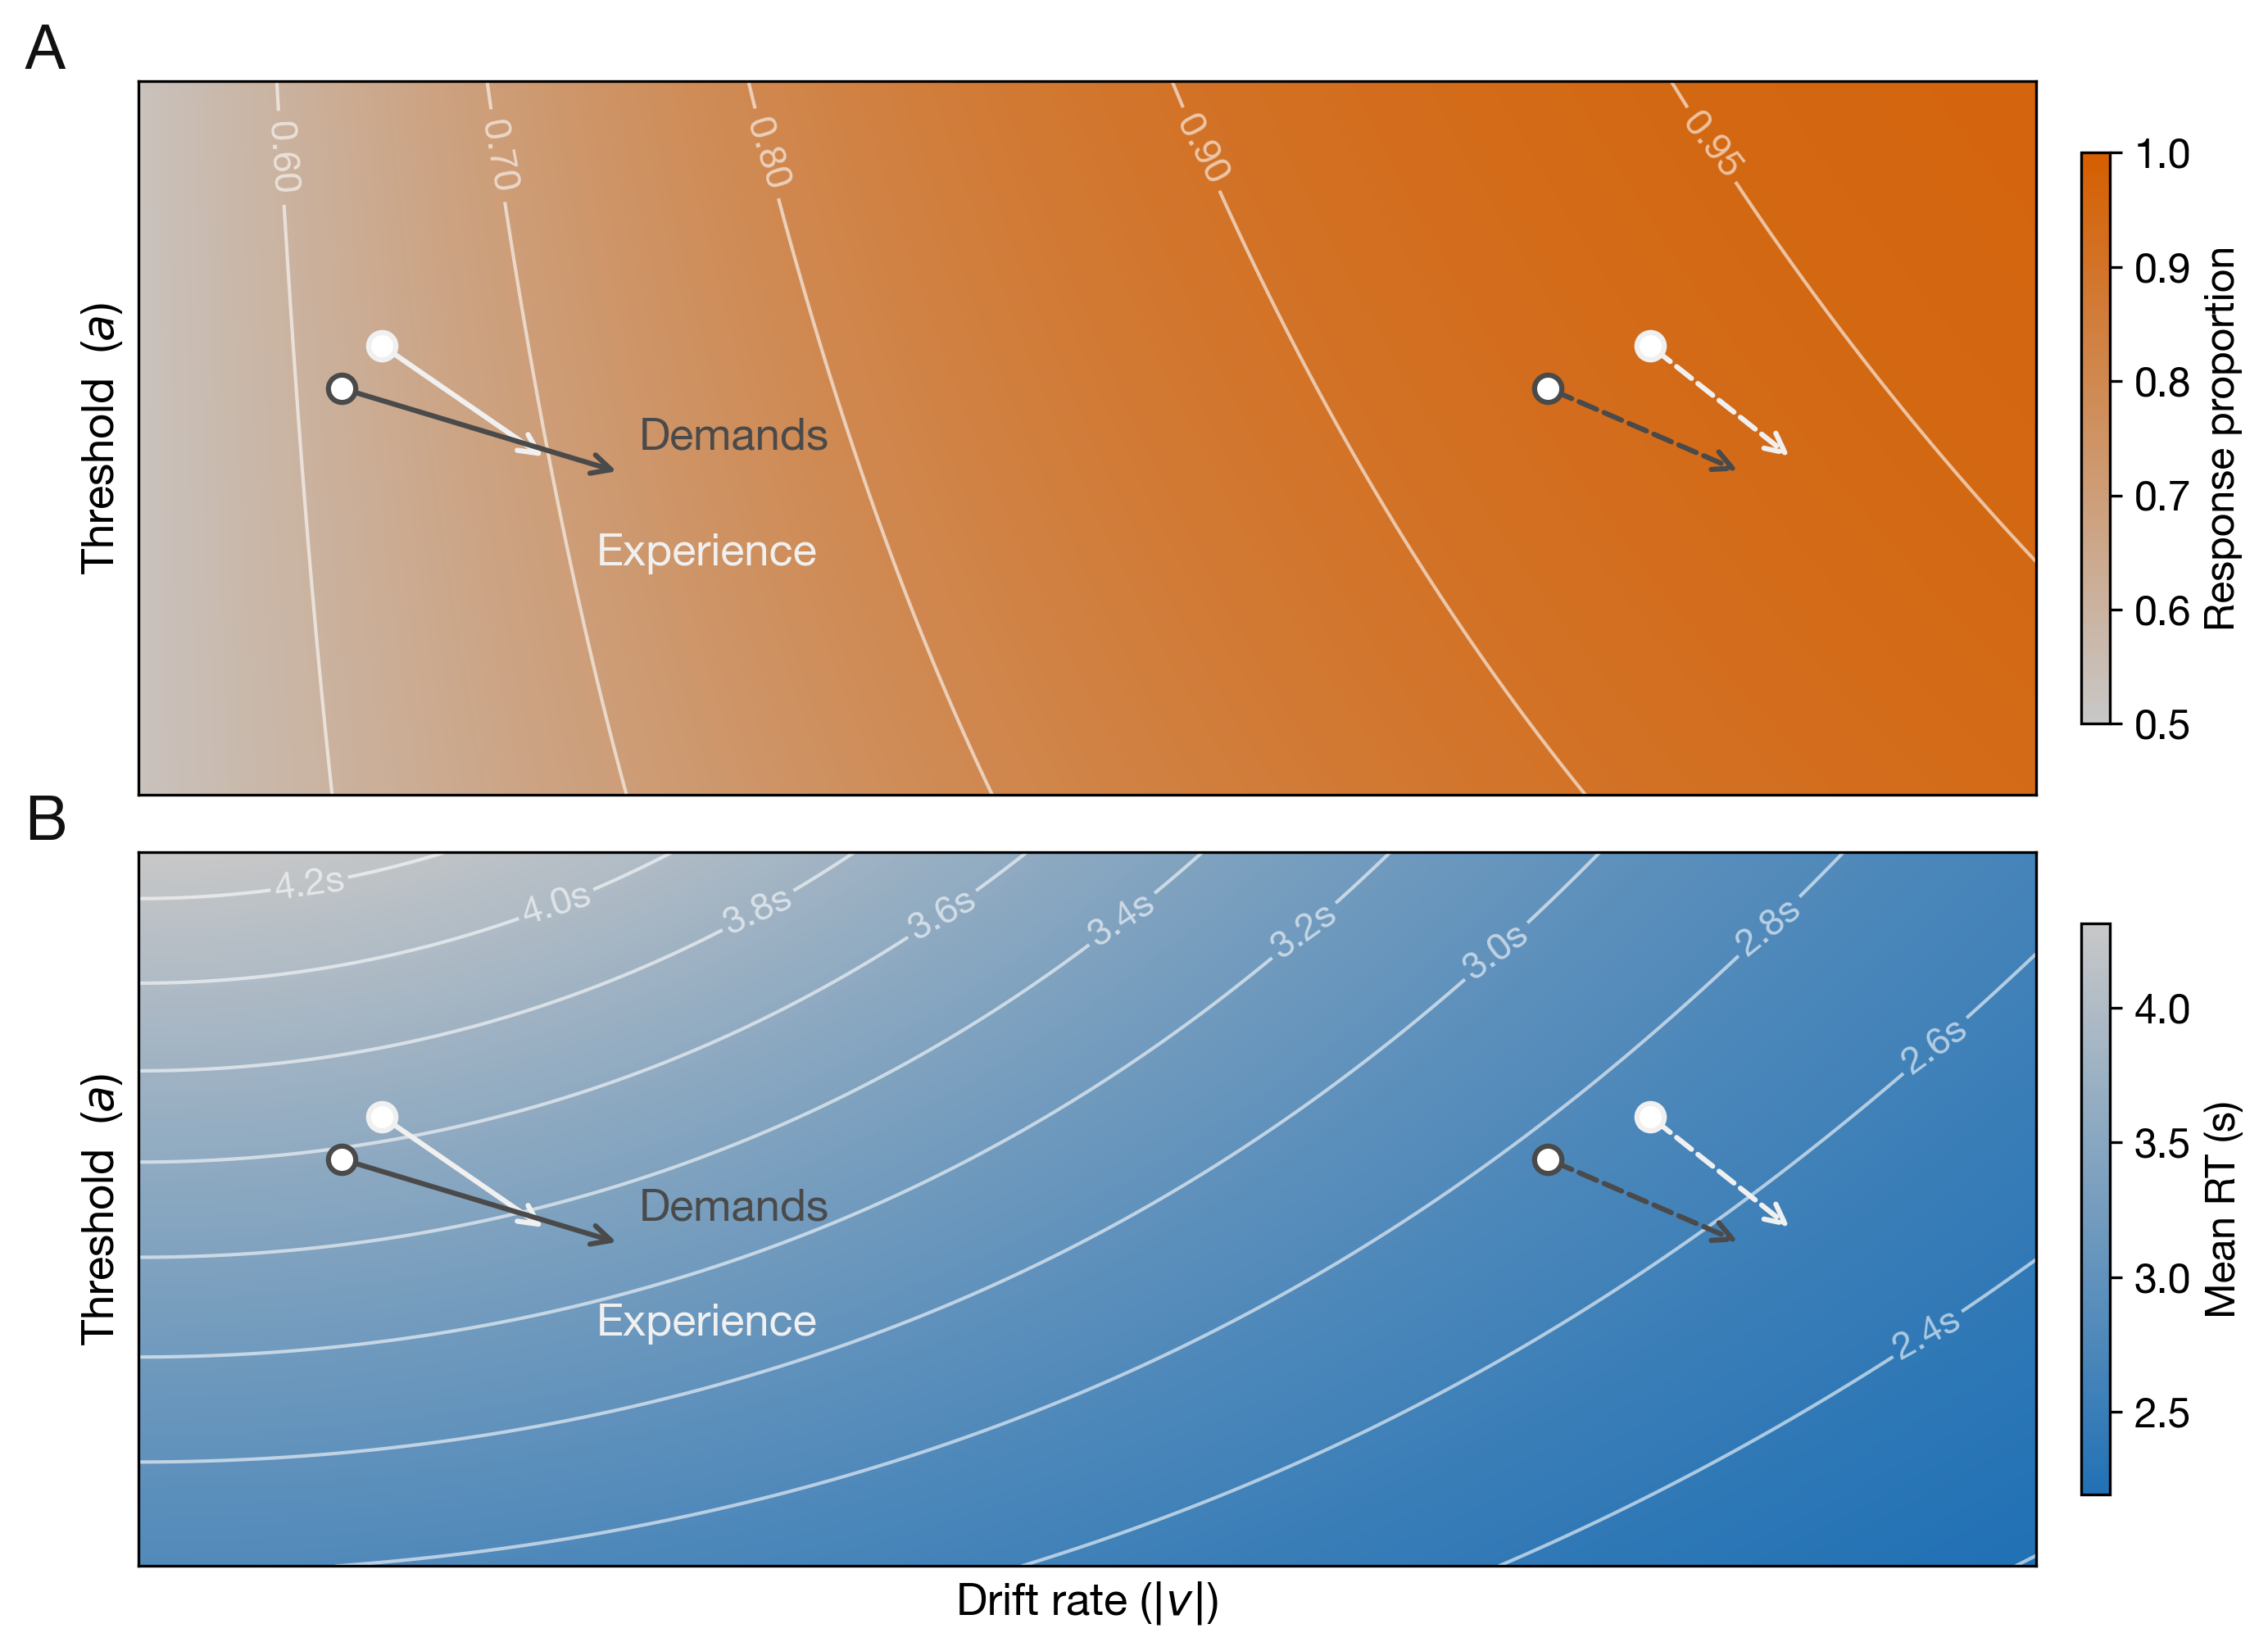
\includegraphics[width=\textwidth]{../figures/Figure6.png}
  \caption{\textbf{DDM Parameter Space with Overlaid Results of Experiment 4b.} Each panel shows mean effective drift rate ($x$-axis) and decision threshold ($y$-axis), with surface color encoding response proportions (top row) and reaction times (bottom row). Heatmaps were computed analytically using closed-form DDM expressions, with a non-decision time of 1~s, a bias of 0.53, and a 5\% contaminant distribution. In the left column, drift rate reflects the difference between text and purpose components. Accordingly, response proportions represent textualism on incongruent trials. In the right column, drift rates reflect the sum of the text and purpose components. Accordingly, response proportions index overall accuracy on congruent trials. Arrows indicate the trajectory of empirical parameter estimates from the pre-block (circle) to the post-block (arrowhead) for the Task Experience and Executive Demand conditions. Both treatments produced increases in drift rate and reductions in decision threshold, indicating faster and more textualist responding over time. Congruent trial accuracy remained near ceiling throughout, suggesting that the drift toward textualism did not impair performance when textual and purposive cues agreed.}
  \label{fig:param_space}
\end{figure}

To understand how the threshold and effective drift rate contributed to strategic reductions in effort (i.e., reaction times) and textualist responses, we calculated the predicted reaction times and rates of textualism in the neighborhood of observed parameter estimates. Threshold reductions (i.e., downward movement in Fig.~\ref{fig:param_space}) shortened reaction times, but contributed minimally to increased textualism. Increases in textualism were primarily due to changes in the net drift rate (i.e., ($v_\text{text} - v_\text{purpose}$)).

%%=============================================================%%
\section{Discussion}\label{sec:discussion}
%%=============================================================%%

Written laws have been argued to constitute a universal element of modern human societies\cite{ref23,ref24,ref25}, serving the purpose of advancing the lawmaker's goals through concrete obligations and prohibitions. Though the enforcement of legal texts often fulfills its underlying purpose\cite{ref26,ref27,ref28}, they also occasionally defy them\cite{ref3,ref8,ref29}. In these circumstances, rule interpretation engenders cognitive conflict and people often prioritize a textualist interpretive policy when they must choose whether to enforce the letter or the spirit of a rule\cite{ref30,ref31,ref32,ref33,ref34}.

The present studies sought to understand why textualist rule enforcement might arise---even at the expense of competing considerations. Doctrinal answers to this question emphasize cultural explanations for the popularity of textualist interpretation, citing precedent, legal education and the like. Here, we tested two psychological explanations, the deliberation and adaptation hypotheses, rooted in widespread models of human cognition,i.e., dual-process and bounded rationality\cite{ref10,ref35,ref36} models, respectively. 

The deliberation hypothesis posited that deliberation promotes textualism by allowing decision-makers to override intuitive, purposive inclinations in favor of more effortful, but accurate, textualist judgments. Thus, participants would prioritize the text when encouraged to exercise greater response caution. We induced greater response caution in two ways, by allowing extra time to do a fixed amount of work and by giving participants less work to do in the same amount of time. Contrary to the deliberation model, neither manipulation increased textualist enforcement. Instead, deliberation appeared to strengthen textualist and purposivist inclinations equally, resulting in no observable change on cases producing letter vs.\ spirit conflict. 

Inspired by evidence that legal officials espouse textualism to a greater extent than the general population, we proposed the adaptation hypothesis: With experience enforcing rules, people shift toward a more computationally efficient, textualist policy. In support of this, we found that textualism did, in fact, increase with task experience---both in an \textit{interim} analysis of our opening studies and in two pre-registered replications. The DDM helped to characterize this shift as the result of reallocating attention from the purpose to the text, producing faster evidence accumulation overall, and lowering the evidence threshold. Exogenous cognitive demands produced the same pattern of adaptations and, importantly, these adaptations preserved accuracy on low-difficulty trials. This suggests that it is not strictly learning from rule enforcement dilemmas, but the exertion and demands on cognitive control they impose, that suffice to strengthen textualist inclinations\cite{ref37}.

Proponents of textualism have argued that adherence to the ordinary meaning of rules helps minimize disagreements among decision-makers\cite{ref38,ref39}. Evidence from a two-player coordination game supports this explanation: People are more likely to converge on textualist verdicts when incentivized to match an anonymous partner's decision than when deciding privately\cite{ref8}. This implies that textualism may allow ``like cases to be treated alike''\cite{ref40,ref41} partly by exploiting a focal point\cite{ref40} among uncommunicated interpreters of a rule. Our present studies offer a complementary explanation for textualism, as a manifestation of the broader phenomenon that people optimize mental effort in response to cognitive demands. Whether these explanations themselves might be related poses an intriguing question for future research: For example, textualism might emerge as a focal point partly because individual decision-makers seek to optimize the trade-off between effort and perceived accuracy by adopting a textualist interpretive policy.

Three limitations merit mention. First, we observed an unexpected reversal of the typical congruency proportion effect on the evidence threshold---with a higher threshold for high- rather than low-congruency blocks of the rule task. One possibility is that participants ``noticed'' evidence accumulating more quickly in high-congruency blocks. If so, they could afford to set a higher threshold without incurring substantial delays. By increasing the evidence threshold when drift rates are high, participants may have strategically traded speed for greater accuracy, producing the observed reversal of the typical congruency-proportion effect. Second, while behavioral effects were evident when analyzed trial-by-trial, they were weaker across larger blocks of trials, suggesting that adaptation may occur rapidly and nonlinearly. Future work may better account for this pattern by modeling these dynamics in a reinforcement learning framework. Third, our studies were modeled after speeded response paradigms in which participants are instructed to decide within a time limit. This approach might raise the concern that our results do not bear on real-world judicial reasoning. However, it has been repeatedly shown that lower-court judges carry excess workloads and must rely on shortcuts to meet administrative demands under severe time constraints\cite{ref42,ref43,ref44,ref45}---a fact that may largely assuage concerns about external validity.

Our studies exploited a fruitful analogy between letter vs.\ spirit conflicts in rule enforcement and lower-level forms of response competition. In so doing, we found that adherence to the letter of the law may provide a solution to the cognitive demands of rule enforcement---one that preserves accuracy while reducing mental work\cite{ref46,ref47}. More broadly, they illustrate how the drift diffusion model can yield a deeper understanding of social reasoning tasks that, like rule interpretation, involve competition between sources of value.

%%=============================================================%%
\section{Methods}\label{sec:methods}
%%=============================================================%%

The experiments were developed in jsPsych (\url{https://www.jspsych.org/7.3/}), and hosted on Cognition (\url{https://www.cognition.run/}). All eight experiments were preregistered: \url{https://researchbox.org/3227\&PEER\_REVIEW\_passcode=AHEJAU}. Participants were recruited on Prolific (\url{www.Prolific.com}) and compensated in accordance with the recommended hourly rate of £10 per hour. The studies were conducted with approval from the Ethics Committee for Research with Humans of the University of Granada (4992/CEIH/2025). Data were analyzed using the R (for behavioral data analysis) and Python (for drift-diffusion modeling) programming languages. Study materials, anonymized data, and analysis scripts for all experiments are available in the project repository at \url{https://osf.io/v35xj/overview?view\_only=865d3fc555bd479cb597a0832a9f1c56}. For all studies, bootstrap power analyses were conducted, by sampling from pilot data with replacement, to establish the required sample size that would suffice to detect the hypothesized effects with power above 90\% at an alpha level of 0.05.

\subsection{Experiments 1a, 1b, and 1c: Violation, compliance and punishment}\label{subsec:exp1}

Experiments 1a and 1b were identical in every respect, except for the test question (``Did this person violate the rule?'' vs.\ ``Did this person comply with the rule?''). In Experiment 1c, we added the description of a punishment to each scenario (e.g., for the ``No shoes in the house'' rule, the corresponding punishment was: ``Anyone found violating the rule will be asked to leave the house''). Participants' task was to indicate for each trial whether the punishment should be applied (e.g., ``Should this person be asked to leave the house?'') instead of whether the behavior violated or complied with the rule.

\paragraph{Participants.}
119 participants completed Experiment 1a ($M_\text{age} = 35.9$, $\mathit{SD}_\text{age} = 14.0$ years, 48\% women, 39\% men, 13\% non-binary or no answer), 124 participants completed Experiment 1b ($M_\text{age} = 36.08$, $\mathit{SD}_\text{age} = 12.3$ years, 49\% women, 48\% men, 3\% non-binary or no answer), and 121 participants completed Experiment 1c ($M_\text{age} = 34.16$, $\mathit{SD}_\text{age} = 11.67$ years, 50\% women, 49\% men, 1\% non-binary or no answer). Inclusion criteria (for all experiments reported in this paper) were: being a native English speaker, not having participated in previous studies using similar materials, and an approval rate of at least 90\% on previous tasks on the platform. Participants received a compensation of £1.50 for an estimated ten minutes of their time.

\paragraph{Design and Procedure.}
We used a 2 (text: violation vs.\ compliance) $\times$ 2 (purpose: violation vs.\ compliance) $\times$ 3 (items) $\times$ 8 (rules) design, with all manipulations administered within participants. Thus, each subject saw 12 trials in each of the 8 scenario blocks, for a total of 96 trials. The order of scenario blocks and trials within blocks was randomized.

Each block began with the presentation of a rule's text and its purpose, e.g.: ``To keep her house clean, Mary announced: No one may wear shoes in the house.'' On the following pages, participants were presented with twelve behaviors (one per page) that either violated the rule's text (literal violation; e.g., ``A guest wears his new sneakers and the floor stays clean''), its purpose (literal compliance; e.g., ``A barefoot guest has a bleeding toe and stains the carpets''), both (violation; e.g., ``A guest wears muddy sneakers and dirties the carpets''), or neither (e.g., ``A guest walks around barefoot and keeps the carpet clean''). On each page, we asked ``Did this person violate the rule?'', and participants were instructed to answer ``Yes'' or ``No'' as soon as they were ready by pressing either the E key or the I key on their keyboard. Assignment of response keys to responses was counterbalanced across participants. Participants had 8 seconds to provide a response, and we recorded responses and reaction times from the display of the target behavior. After a time limit of 8 seconds without a response, a trial was recorded as invalid. A fixation cross was presented between trials with a randomized duration between 250 and 2,000~ms.

Before the main experiment, participants completed a practice block involving a prohibition on noise at night (without time pressure or incongruent trials) to familiarize themselves with the layout and task. Participants had the opportunity to take a break after each block. The experiment concluded with the assessment of demographic variables, including age, gender, and handedness, followed by a debriefing.

\paragraph{Analysis.}
We conducted a mixed-effects logistic regression of rule violation judgments, with text, purpose and the text$\times$purpose interactions as fixed effects (and scenarios and participants as crossed, random effects) in the \texttt{lme4} package. We also conducted a mixed-effects regression of response times, with text, purpose and the text$\times$purpose interactions as fixed effects (and scenario and participant as crossed random effects).

We ran a series of drift diffusion models in the \texttt{hddm} library\cite{ref16} in Python, with an outlier probability of 5\% to account for lapses in attention or extreme responses. Posterior distributions were sampled using Markov Chain Monte Carlo (MCMC) with 10,000 samples, a burn-in of 10\% of the samples, and thinning every 3 samples. Drift rates ($v$) and non-decision times ($t$) were allowed to vary across experimental conditions, while threshold ($a$) and bias ($z$) were kept constant across conditions. We forced a constant threshold across case-types, under the assumption that participants would not adjust their degree of response caution flexibly on each trial, given that trial type was randomized and thus unpredictable. We predicted that (1) the model with a $z$ term would improve fit to the data relative to a model without $z$, and that (2) the model allowing $v$ to vary across conditions would improve fit to the data relative to a model in which $v$ is constant across conditions. We compared model fit on the basis of the Deviance Information Criterion. Posterior predictive checks comparing observed data to simulated data drawn from the model's posterior parameter estimates revealed satisfactory fit to the data (see Supplementary Analysis~\hyperref[supp:analysis4]{4}).

\subsection{Experiment 2: Cross-task correlations}\label{subsec:exp2}

\paragraph{Participants.}
301 participants completed the study ($M_\text{age} = 43.9$, $\mathit{SD}_\text{age} = 15.6$ years, 50\% women, 49\% men, 1\% non-binary or no answer) and received £2.40 as compensation for an estimated 16 minutes of their time. Given evidence of age differences in diffusion model parameters\cite{ref48}, we sought to avoid range restriction by applying a stratified sampling procedure with five age bands: 18--28, 29--39, 40--51, 52--63, and 64--89 years.

\paragraph{Design and Procedure.}
Design, procedure and materials for the rules task were identical to those used in Experiment 1a. However, the eight scenarios about rules were now interspersed with blocks of Stroop and Flanker tasks (four blocks each) in a randomized order.

In the Stroop task, we presented 24 trials per block. Each block included 12 congruent trials, in which the color word (e.g., ``green'') was printed in the corresponding color, and 12 incongruent trials, in which the color word and text color did not match (e.g., the word ``green'' printed in red). Participants' task was to indicate the text color as quickly as possible by pressing the letters ``R'' (for red), ``B'' (for blue), ``G'' (for green), or ``Y'' (for yellow) on their keyboard. The stimuli were sampled with replacement from a list containing all 16 pairings of color word and text color. Each of the 24 stimuli was presented once per block, and the order of presentation was randomized. Participants had three seconds to provide a response, which terminated the trial, and each trial was preceded by a fixation cross with a variable duration between 250 and 1750~ms. No feedback on response accuracy was provided.

In the Flanker task, we also presented 24 trials per block. Each block included 12 congruent trials, in which the middle arrow pointed in the same direction as the flanking arrows (e.g., $<\!<\!<\!<\!<$ or $>\!>\!>\!>\!>$), and 12 incongruent trials, in which the middle arrow pointed in the opposite direction to the flanking arrows (e.g., $<\!<\!>\!<\!<$ or $>\!>\!<\!>\!>$). Participants' task was to indicate the direction of the middle arrow as quickly as possible by pressing ``E'' for left-pointing arrows or ``I'' for right-pointing arrows on their keyboard. Participants had 1.5 seconds to provide a response, and each trial was preceded by a fixation cross with a variable duration between 250 and 1750~ms. No feedback on response accuracy was provided.

All in all, participants completed 96 rule trials (8 blocks of 12 trials), 96 Stroop trials (4 blocks of 24 trials), and 96 Flanker trials (4 blocks of 24 trials) in this experiment, and were free to take a break between blocks.

At the end of the experiment, participants were asked two questions aimed to capture individual differences in rule interpretation preferences. The first question asked: ``Which of the following statements better captures your belief about what it means to violate or comply with a rule?'' Participants were given two response options: (i) ``To abide by the law, one must focus on the letter of the law. So, when someone acts in a way that conflicts with a rule's text (what it literally says), then that person has broken the rule.'' (ii) ``To abide by the law, one must focus on the spirit of the law. So, when someone acts in a way that conflicts with a rule's purpose (what it is ultimately for), then that person has broken the rule.'' Then participants rated the extent to which they relied on each approach on a 7-point Likert scale. The experiment ended with the assessment of demographic variables and a debriefing.

\paragraph{Analysis.}
We first analyzed the pattern of interference effects on accuracy and reaction times on each task, with a fixed effect of trial type (congruent vs.\ incongruent) into baseline models with only a random intercept for participant (and a second random intercept for scenario in the rules task).

We fit hierarchical drift diffusion models using the \texttt{hddmRegressor} function to each task. To facilitate comparison across them, we used the same model specification for every task allowing the $v$ parameter (drift rate) to vary between congruent and incongruent trials. We assessed the pattern of correlations between participant-level parameter estimates across tasks. Prior to the correlation analysis, we excluded multivariate outliers by calculating the Mahalanobis distance for each set of parameter estimates, and excluding estimates with a probability $< .001$ of belonging to the multivariate distribution.

We then conducted a bifactor confirmatory analysis using the \texttt{lavaan} package\cite{ref49} to assess the degree of commonality versus specificity in drift diffusion parameters across tasks. The model specified one general and three orthogonal specific factors, with each item loading on the general factor and one specific factor. Parameters were estimated using maximum likelihood (ML) and latent variables were identified by fixing the first loading of each latent factor to 1.

\subsection{Experiment 3a: Speed vs.\ accuracy instructions}\label{subsec:exp3a}

\paragraph{Participants.}
123 participants completed the study ($M_\text{age} = 35.6$, $\mathit{SD}_\text{age} = 11.0$ years, 50\% women, 50\% men) and received £1.50 as compensation for an estimated ten minutes of their time.

\paragraph{Design and Procedure.}
Design, materials, and procedure were identical to Experiment 1a with the addition of a within-subjects, speed-accuracy manipulation. In four of the eight scenarios, participants were instructed to prioritize accuracy over speed (10-second time limit); in the other four scenarios, they were instructed to prioritize speed (5-second time limit). Each participant received four consecutive blocks in accuracy mode and four consecutive blocks in speed mode, in a counterbalanced order across participants.

\paragraph{Analysis.}
We conducted a mixed-effects logistic regression of violation judgments, with mode, text, purpose and every two- and three-way interaction as fixed effects. We also conducted a series of hierarchical drift diffusion models, predicting that a model allowing the evidence threshold to vary as a function of speed vs.\ accuracy mode would improve fit to the data, using lower DIC as the decision criterion.

\subsection{Experiment 3b: Proportion of congruency manipulation}\label{subsec:exp3b}

\paragraph{Participants.}
121 participants completed the survey ($M_\text{age} = 35.2$, $\mathit{SD}_\text{age} = 13.3$ years, 51\% women, 48\% men, 1\% non-binary or no answer) and received £1.50 as compensation for an estimated ten minutes of their time.

\paragraph{Design and Procedure.}
Design, materials, and procedure were identical to Experiments 1a and 1b except for an additional within-subjects manipulation of the proportion of congruent vs.\ incongruent trials per scenario. Participants completed two blocks: a block with a high proportion of congruent trials (10 out of 12 trials per scenario) and another block with a low proportion of congruent trials (2 out of 12 trials per scenario). The order of the congruency proportion blocks was randomized between subjects.

\paragraph{Analysis.}
We conducted a mixed-effects logistic regression of violation judgments, with congruency proportion, text, purpose, and every two- and three-way interaction as fixed effects. We also conducted hierarchical drift diffusion models, predicting that a model allowing the evidence threshold to vary as a function of congruency proportion would improve fit.

\subsection{Experiment 4a: Task experience vs.\ executive demands (between-subjects)}\label{subsec:exp4a}

\paragraph{Participants.}
227 participants completed the study ($M_\text{age} = 39.2$, $\mathit{SD}_\text{age} = 12.7$ years, 50\% women, 49\% men, $<$1\% non-binary or no answer) and received £1.50 as compensation for an estimated ten minutes of their time.

\paragraph{Design and Procedure.}
Participants were randomly assigned to one of two between-subjects conditions: Task Experience or Executive Demand. In the Task Experience condition, participants completed all 8 blocks of the rules task. In the Executive Demand condition, participants first completed 2 blocks of Stroop and 2 blocks of Flanker tasks (in a randomized order), followed by 4 blocks of the rules task. Thus, both groups participated in four blocks of an identical rules task; the between-subjects manipulation concerned whether participants had previously completed four baseline blocks of the same rules task (Task Experience) or four blocks of Stroop and Flanker tasks (Executive Demand).

\paragraph{Analysis.}
We min-max normalized trial number and tested whether it moderated the effects of text and purpose on violation judgments in a mixed-effects logistic regression. In the Task Experience condition, we labeled the first four blocks as the baseline (Rules$_0$), the last four blocks as the post-task experience block (Rules$_E$). In the Executive Demand condition, we labeled the four blocks as the post-executive demands block (Rules$_D$). We fit hierarchical drift diffusion models using the \texttt{hddmRegressor} function to assess whether block (Rules$_0$, Rules$_D$, Rules$_E$) influenced the drift rates of text and purpose, thresholds, and/or non-decision times.

\subsection{Experiment 4b: Task experience vs.\ executive demands (pre-to-post change)}\label{subsec:exp4b}

\paragraph{Participants.}
600 participants completed Experiment 4b ($M_\text{age} = 46.9$, $\mathit{SD}_\text{age} = 25.2$ years, 50\% women, 49\% men, 1\% non-binary or no answer) and received £1.50 as compensation for an estimated ten minutes of their time.

\paragraph{Design and Procedure.}
Participants were randomly assigned to one of three treatment conditions with equal probability: Passive Control (viewing a 3-minute time lapse video), Executive Demand (4 blocks of Stroop and Flanker tasks), or Task Experience (4 blocks of the Rules task). In every condition, participants completed a pre-treatment block of the Rules task, followed by the randomly assigned treatment, and a post-treatment block of the Rules task. The pre- and post-blocks contained two rules each, with 12 trials per rule (24 trials each).

\paragraph{Analysis.}
Applying forward model selection, we compared a series of mixed-effects logistic regression models to a baseline model with only main effects of text and purpose. Model 1 allowed block (pre vs.\ post) to interact with both text and purpose factors. In Models 2a, 2b, and 2c, we specified the same model and ran it on each treatment condition separately. According to the learning hypothesis, the interaction should emerge in Model 2a only. According to the effort hypothesis, it should emerge in Models 2a and 2b. With the \texttt{hddmRegressor} function, we modeled whether pre-to-post changes in the effects of text and purpose were captured by changes in drift rate, non-decision time, and/or threshold, including a fixed bias in the model.

%%=============================================================%%
%% References
%%=============================================================%%

\bibliography{textualism-ddm}

%%=============================================================%%
%% Supplementary Material
%%=============================================================%%

\clearpage
\begin{appendices}

%% Prefix supplementary tables and figures with "S"
\renewcommand{\thetable}{S\arabic{table}}
\renewcommand{\thefigure}{S\arabic{figure}}

\section*{Supplementary Material}

\FloatBarrier

% ============================================================
\subsection*{Supplementary Analysis 1: Logistic model of choice in Studies 1a--c}
\label{supp:analysis1}
% ============================================================

Supplementary Table~\ref{tab:S1} reports the results of mixed-effects logistic regression models of decisions in Studies 1a--c, with random intercepts of participant and scenario. All three models reveal main effects of text and purpose, $p$s $< .001$.


\begin{table}[htbp]
\caption{Logistic regression models of choice (Studies 1a--c).}
\label{tab:S1}
\begin{tabular*}{\textwidth}{@{\extracolsep{\fill}}lrrrrl}
\toprule
Predictor & OR & 2.5\% & 97.5\% & $z$ & $p$ \\
\midrule
\multicolumn{6}{l}{\textit{Study 1a (Did the agent violate the rule?)}} \\
Intercept & 0.04 & 0.03 & 0.05 & $-$28.75 & $<.001$ \\
Text      & 48.23 & 42.09 & 55.27 & 55.78 & $<.001$ \\
Purpose   & 8.53  & 7.47  & 9.74  & 31.71 & $<.001$ \\
\midrule
\multicolumn{6}{l}{\textit{Study 1b (Did the agent comply with the rule?)}} \\
Intercept & 12.60 & 10.67 & 14.88 & 29.86 & $<.001$ \\
Text      & 0.03  & 0.03  & 0.04  & $-$42.55 & $<.001$ \\
Purpose   & 0.22  & 0.19  & 0.26  & $-$18.41 & $<.001$ \\
\midrule
\multicolumn{6}{l}{\textit{Study 1c (Should the agent be punished?)}} \\
Intercept & 0.05  & 0.035 & 0.06  & $-$23.07 & $<.001$ \\
Text      & 14.65 & 12.97 & 16.54 & 43.30 & $<.001$ \\
Purpose   & 18.92 & 16.74 & 21.38 & 47.17 & $<.001$ \\
\bottomrule
\end{tabular*}
\footnotetext{OR = odds ratio. Random effects: participant and scenario (crossed).}
\end{table}

\clearpage

\FloatBarrier

% ============================================================
\subsection*{Supplementary Analysis 2: Log-linear model of reaction times in Studies 1a--c}
\label{supp:analysis2}
% ============================================================

Supplementary Table~\ref{tab:S2} reports the results of mixed-effects linear regression models of log-transformed reaction times in Studies 1a--c, with random intercepts of participant and scenario. All three models reveal a two-way interaction between text and purpose, $p$s $< .001$---representing the interference effect on reaction times (see also Supplementary Figure~\ref{fig:S1}).

\begin{table}[htbp]
\caption{Linear regression models of log-transformed reaction times (Studies 1a--c).}
\label{tab:S2}
\begin{tabular*}{\textwidth}{@{\extracolsep{\fill}}lrrrrl}
\toprule
Predictor & $B$ & 2.5\% & 97.5\% & $t$ & $p$ \\
\midrule
\multicolumn{6}{l}{\textit{Study 1a}} \\
Intercept              & 7.73  & 7.65  & 7.81  & 189.33  & $<.001$ \\
Text                   & 0.26  & 0.24  & 0.28  & 26.01   & $<.001$ \\
Purpose                & 0.15  & 0.13  & 0.17  & 15.57   & $<.001$ \\
Text $\times$ Purpose  & $-$0.41 & $-$0.43 & $-$0.38 & $-$29.01 & $<.001$ \\
\midrule
\multicolumn{6}{l}{\textit{Study 1b}} \\
Intercept              & 7.73  & 7.64  & 7.82  & 166.22  & $<.001$ \\
Text                   & 0.22  & 0.20  & 0.24  & 21.99   & $<.001$ \\
Purpose                & 0.15  & 0.13  & 0.17  & 14.78   & $<.001$ \\
Text $\times$ Purpose  & $-$0.38 & $-$0.41 & $-$0.36 & $-$26.93 & $<.001$ \\
\midrule
\multicolumn{6}{l}{\textit{Study 1c}} \\
Intercept              & 7.79  & 7.72  & 7.85  & 219.50  & $<.001$ \\
Text                   & 0.25  & 0.23  & 0.27  & 24.59   & $<.001$ \\
Purpose                & 0.18  & 0.16  & 0.20  & 18.02   & $<.001$ \\
Text $\times$ Purpose  & $-$0.42 & $-$0.44 & $-$0.39 & $-$29.47 & $<.001$ \\
\bottomrule
\end{tabular*}
\end{table}

\begin{figure}[htbp]
  \centering
  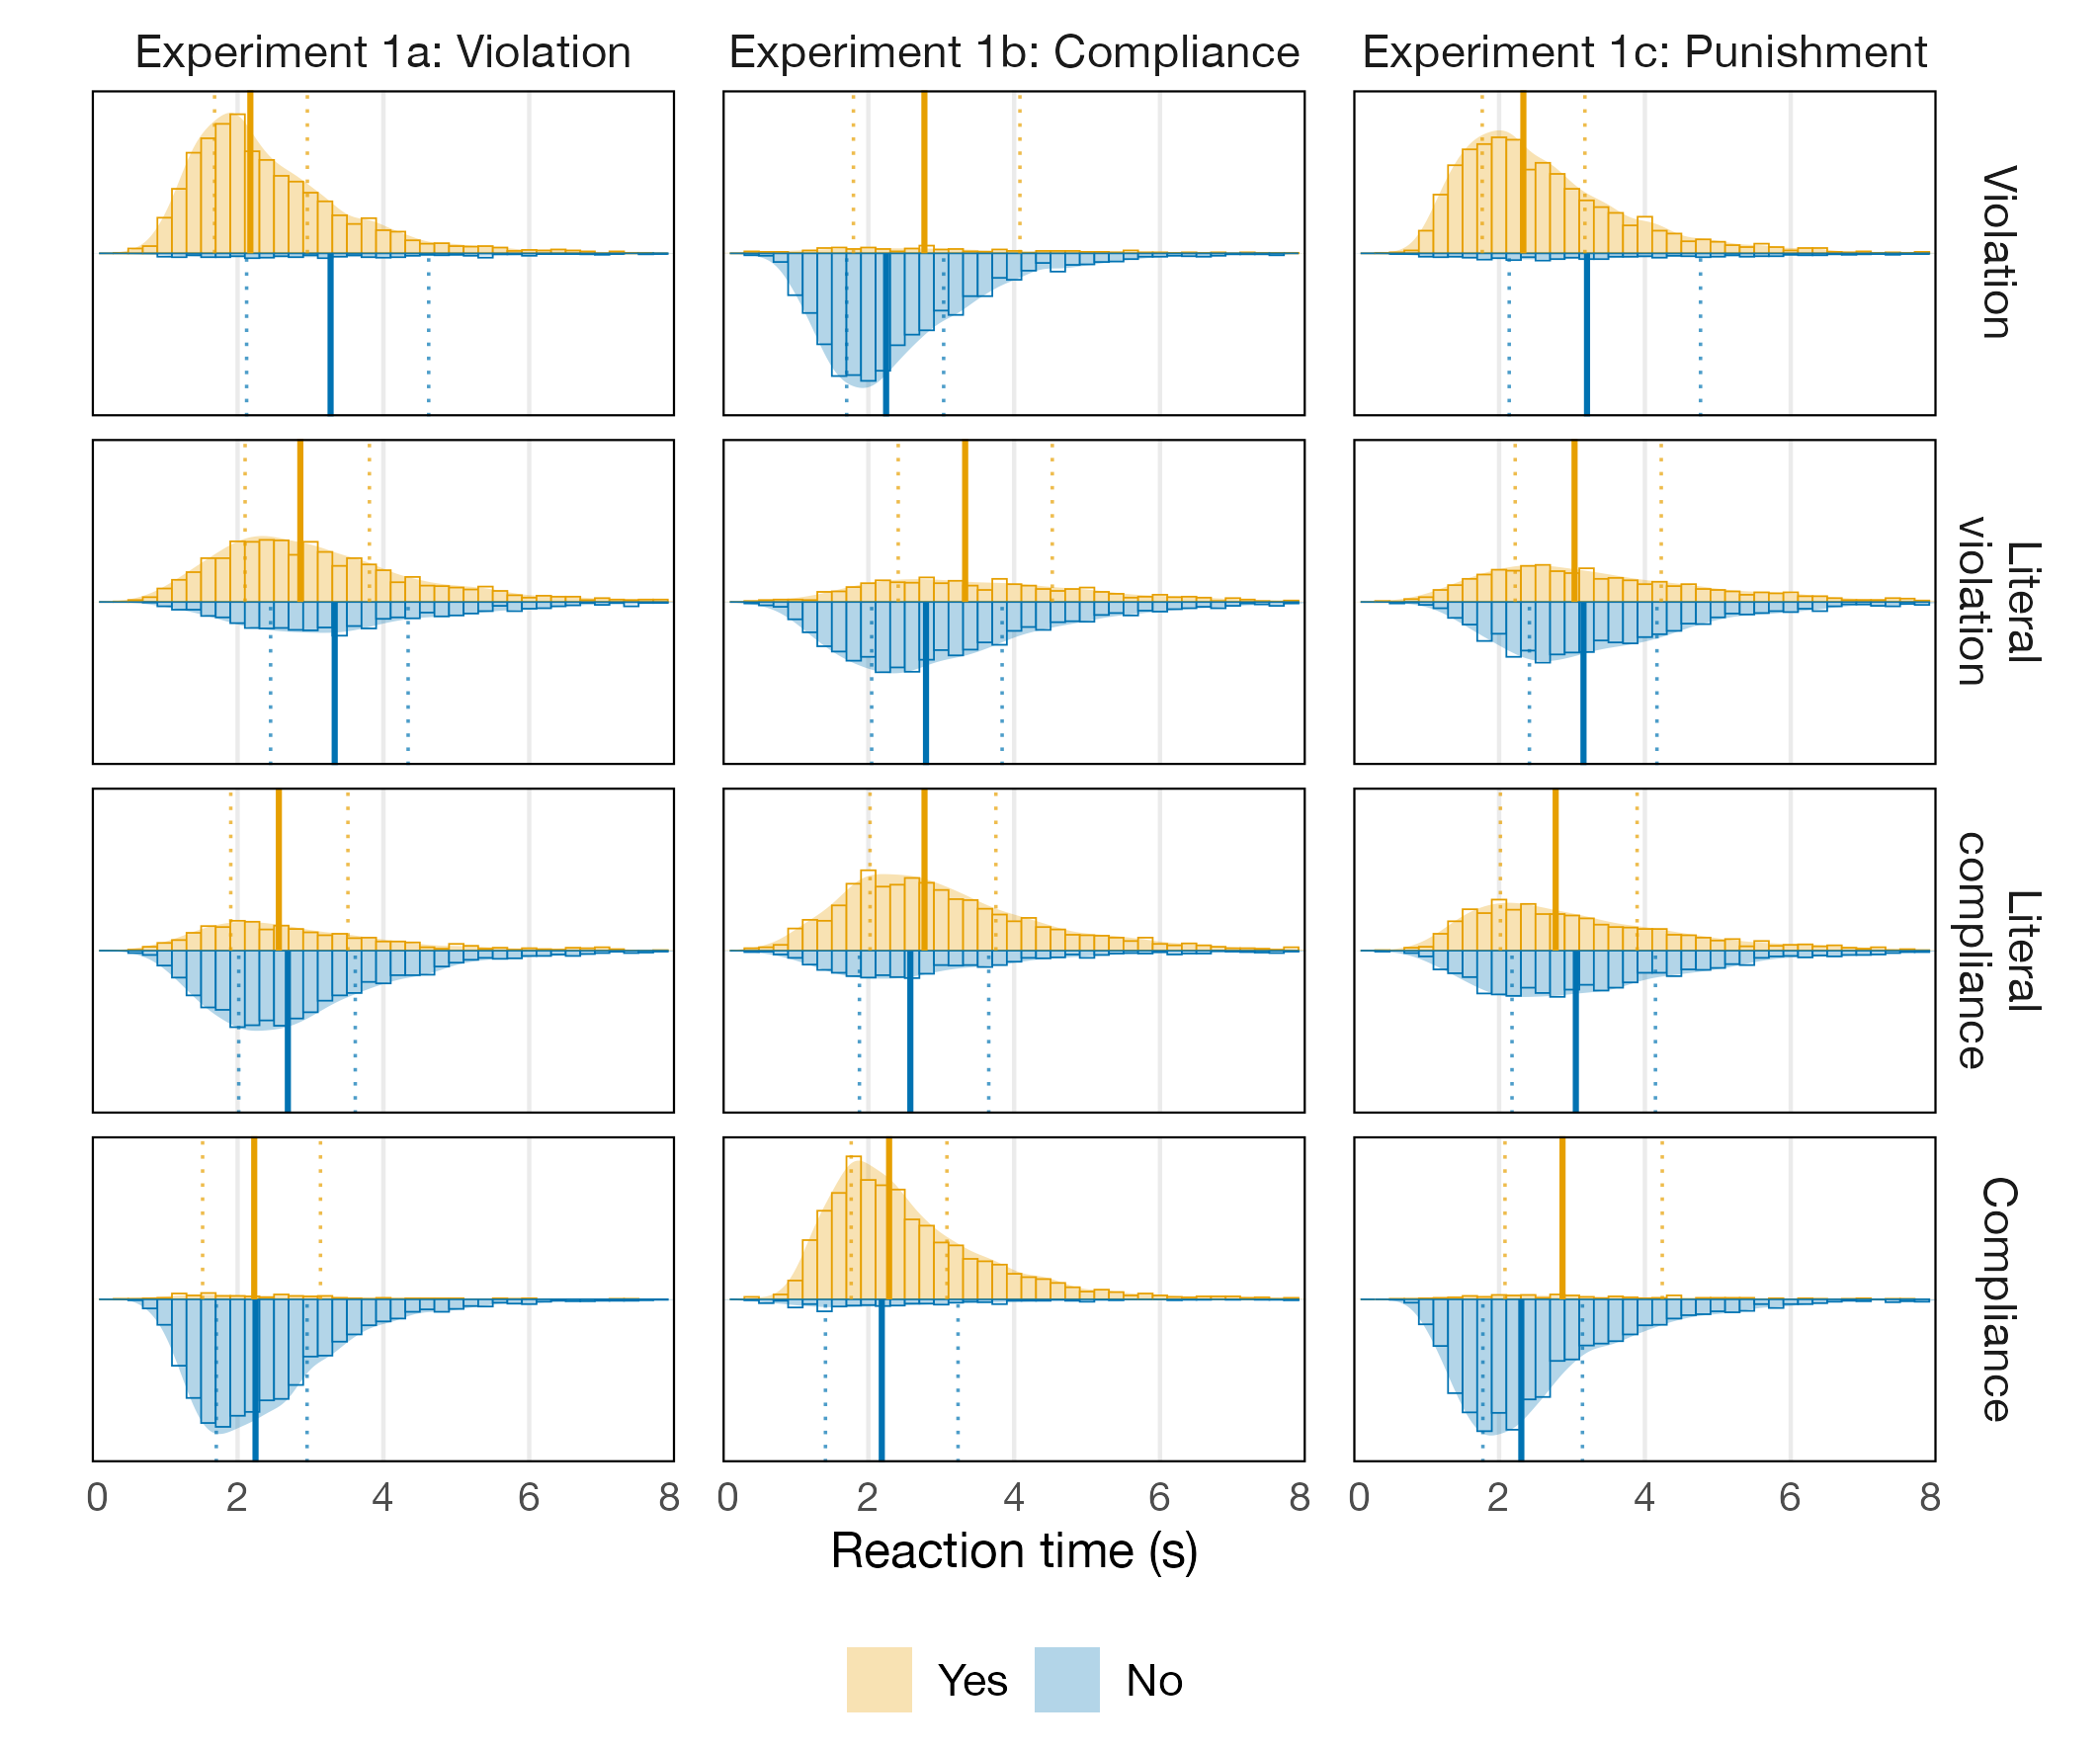
\includegraphics[width=\textwidth]{../figures/SuppFigure1.png}
  \caption{Grouped histograms of reaction times by condition (rows) and study (columns).}
  \label{fig:S1}
\end{figure}

\clearpage

\FloatBarrier

% ============================================================
\subsection*{Supplementary Analysis 3: Drift diffusion models in Studies 1a--c}
\label{supp:analysis3}
% ============================================================

We fit a hierarchical drift-diffusion model to the reaction time and choice data in Studies 1a--c using the \texttt{hddm} package. Drift rates ($v$) and non-decision times ($t$) were modeled as dependent on the experimental conditions text and purpose, allowing these parameters to vary across conditions. Threshold ($a$) and bias ($z$) were estimated as constant across conditions.

We included an outlier probability of 5\% to account for lapses in attention or extreme responses. Posterior distributions were sampled using Markov Chain Monte Carlo with 10,000 samples, a burn-in of 10\% of the samples, and thinning every 3 samples. Results are reported in Supplementary Table~\ref{tab:S3}.

\begin{table}[htbp]
\caption{Hierarchical drift-diffusion model summaries: Studies 1a--c.}
\label{tab:S3}
\raggedright
\begin{tabular*}{\textwidth}{@{\extracolsep{\fill}}lrrr@{}}
\toprule
Parameter & Mean & 2.5\% & 97.5\% \\
\midrule
\multicolumn{4}{l}{\textit{Study 1a}} \\
$a$                      & 3.16  & 3.08  & 3.25  \\
$v$ (compliance)         & $-$1.18 & $-$1.26 & $-$1.11 \\
$v$ (literal compliance) & $-$0.52 & $-$0.59 & $-$0.45 \\
$v$ (literal violation)  & 0.23  & 0.16  & 0.30  \\
$v$ (violation)          & 1.02  & 0.94  & 1.09  \\
$t$ (compliance)         & 1.03  & 0.96  & 1.10  \\
$t$ (literal compliance) & 1.01  & 0.94  & 1.08  \\
$t$ (literal violation)  & 1.17  & 1.10  & 1.25  \\
$t$ (violation)          & 1.05  & 0.98  & 1.11  \\
$z$                      & 0.54  & 0.52  & 0.54  \\
\midrule
\multicolumn{4}{l}{\textit{Study 1b}} \\
$a$                      & 3.23  & 3.11  & 3.36  \\
$v$ (compliance)         & 1.13  & 1.05  & 1.22  \\
$v$ (literal compliance) & 0.55  & 0.47  & 0.62  \\
$v$ (literal violation)  & $-$0.36 & $-$0.44 & $-$0.28 \\
$v$ (violation)          & $-$1.03 & $-$1.11 & $-$0.95 \\
$t$ (compliance)         & 1.04  & 0.97  & 1.12  \\
$t$ (literal compliance) & 1.02  & 0.94  & 1.10  \\
$t$ (literal violation)  & 1.12  & 1.04  & 1.20  \\
$t$ (violation)          & 1.07  & 1.00  & 1.15  \\
$z$                      & 0.46  & 0.45  & 0.47  \\
\midrule
\multicolumn{4}{l}{\textit{Study 1c}} \\
$a$                      & 3.07  & 2.99  & 3.15  \\
$v$ (compliance)         & $-$1.16 & $-$1.24 & $-$1.08 \\
$v$ (literal compliance) & $-$0.11 & $-$0.18 & $-$0.04 \\
$v$ (literal violation)  & $-$0.23 & $-$0.30 & $-$0.16 \\
$v$ (violation)          & 0.90  & 0.82  & 0.97  \\
$t$ (compliance)         & 1.16  & 1.09  & 1.24  \\
$t$ (literal compliance) & 1.22  & 1.14  & 1.30  \\
$t$ (literal violation)  & 1.37  & 1.29  & 1.45  \\
$t$ (violation)          & 1.17  & 1.10  & 1.25  \\
$z$                      & 0.54  & 0.53  & 0.55  \\
\bottomrule
\end{tabular*}
\end{table}

\clearpage

\FloatBarrier

% ============================================================
\subsection*{Supplementary Analysis 4: Posterior predictive checks in Studies 1a--c}
\label{supp:analysis4}
% ============================================================

Model convergence was assessed using the default HDDM diagnostics (see Supplementary Table~\ref{tab:S4}). Posterior predictive checks indicated adequate model fit: all summary statistics fell within 95\% credible intervals. The model accurately recovered observed ``Yes'' and ``No'' rates and the full RT distribution for correct responses across all conditions. Minor misfit in the variance and extreme quantiles of RT distributions occurred in two conditions that represent erroneous responses in congruent cases (see dotted lines in Supplementary Figure~\ref{fig:S2}).

\begin{table}[htbp]
\caption{Convergence diagnostics ($\hat{R}$, bulk and tail effective sample sizes).}
\label{tab:S4}
\begin{tabular*}{\textwidth}{@{\extracolsep{\fill}}llrrr@{}}
\toprule
Parameter & Study & $\hat{R}$ & ESS$_\text{bulk}$ & ESS$_\text{tail}$ \\
\midrule
$a$ & 1a & 1.00 & 1474.37 & 2615.94 \\
    & 1b & 1.00 & 1517.34 & 2419.51 \\
    & 1c & 1.00 & 1938.62 & 2912.78 \\
$t$ (compliance) & 1a & 1.01 & 1132.69 & 2292.01 \\
                  & 1b & 1.00 & 1795.83 & 2341.23 \\
                  & 1c & 1.00 & 1599.37 & 2638.41 \\
$t$ (literal violation) & 1a & 1.00 & 1678.52 & 2516.85 \\
                         & 1b & 1.00 & 2232.32 & 2779.98 \\
                         & 1c & 1.00 & 2108.52 & 2731.58 \\
$t$ (literal compliance) & 1a & 1.00 & 2032.49 & 2619.35 \\
                          & 1b & 1.00 & 2231.87 & 2715.98 \\
                          & 1c & 1.00 & 1977.61 & 2682.99 \\
$t$ (violation) & 1a & 1.01 & 1895.66 & 2731.10 \\
                 & 1b & 1.00 & 2727.42 & 2715.79 \\
                 & 1c & 1.00 & 1551.64 & 2752.53 \\
$v$ (compliance) & 1a & 1.01 & 262.50  & 2466.05 \\
                  & 1b & 1.00 & 1869.34 & 2756.17 \\
                  & 1c & 1.00 & 959.25  & 1934.36 \\
$v$ (literal violation) & 1a & 1.01 & 485.53  & 1657.23 \\
                         & 1b & 1.00 & 1409.05 & 2465.79 \\
                         & 1c & 1.01 & 195.43  & 2160.13 \\
$v$ (literal compliance) & 1a & 1.01 & 302.16  & 1874.86 \\
                          & 1b & 1.00 & 1722.77 & 2721.78 \\
                          & 1c & 1.00 & 471.54  & 2394.39 \\
$v$ (violation) & 1a & 1.01 & 495.62  & 1038.77 \\
                 & 1b & 1.00 & 1542.01 & 2519.15 \\
                 & 1c & 1.01 & 462.78  & 1796.64 \\
$z$ & 1a & 1.22 & 3.66    & 27.20   \\
    & 1b & 1.00 & 64.05   & 150.50  \\
    & 1c & 1.06 & 11.09   & 65.19   \\
\bottomrule
\end{tabular*}
\end{table}

\begin{figure}[htbp]
  \centering
  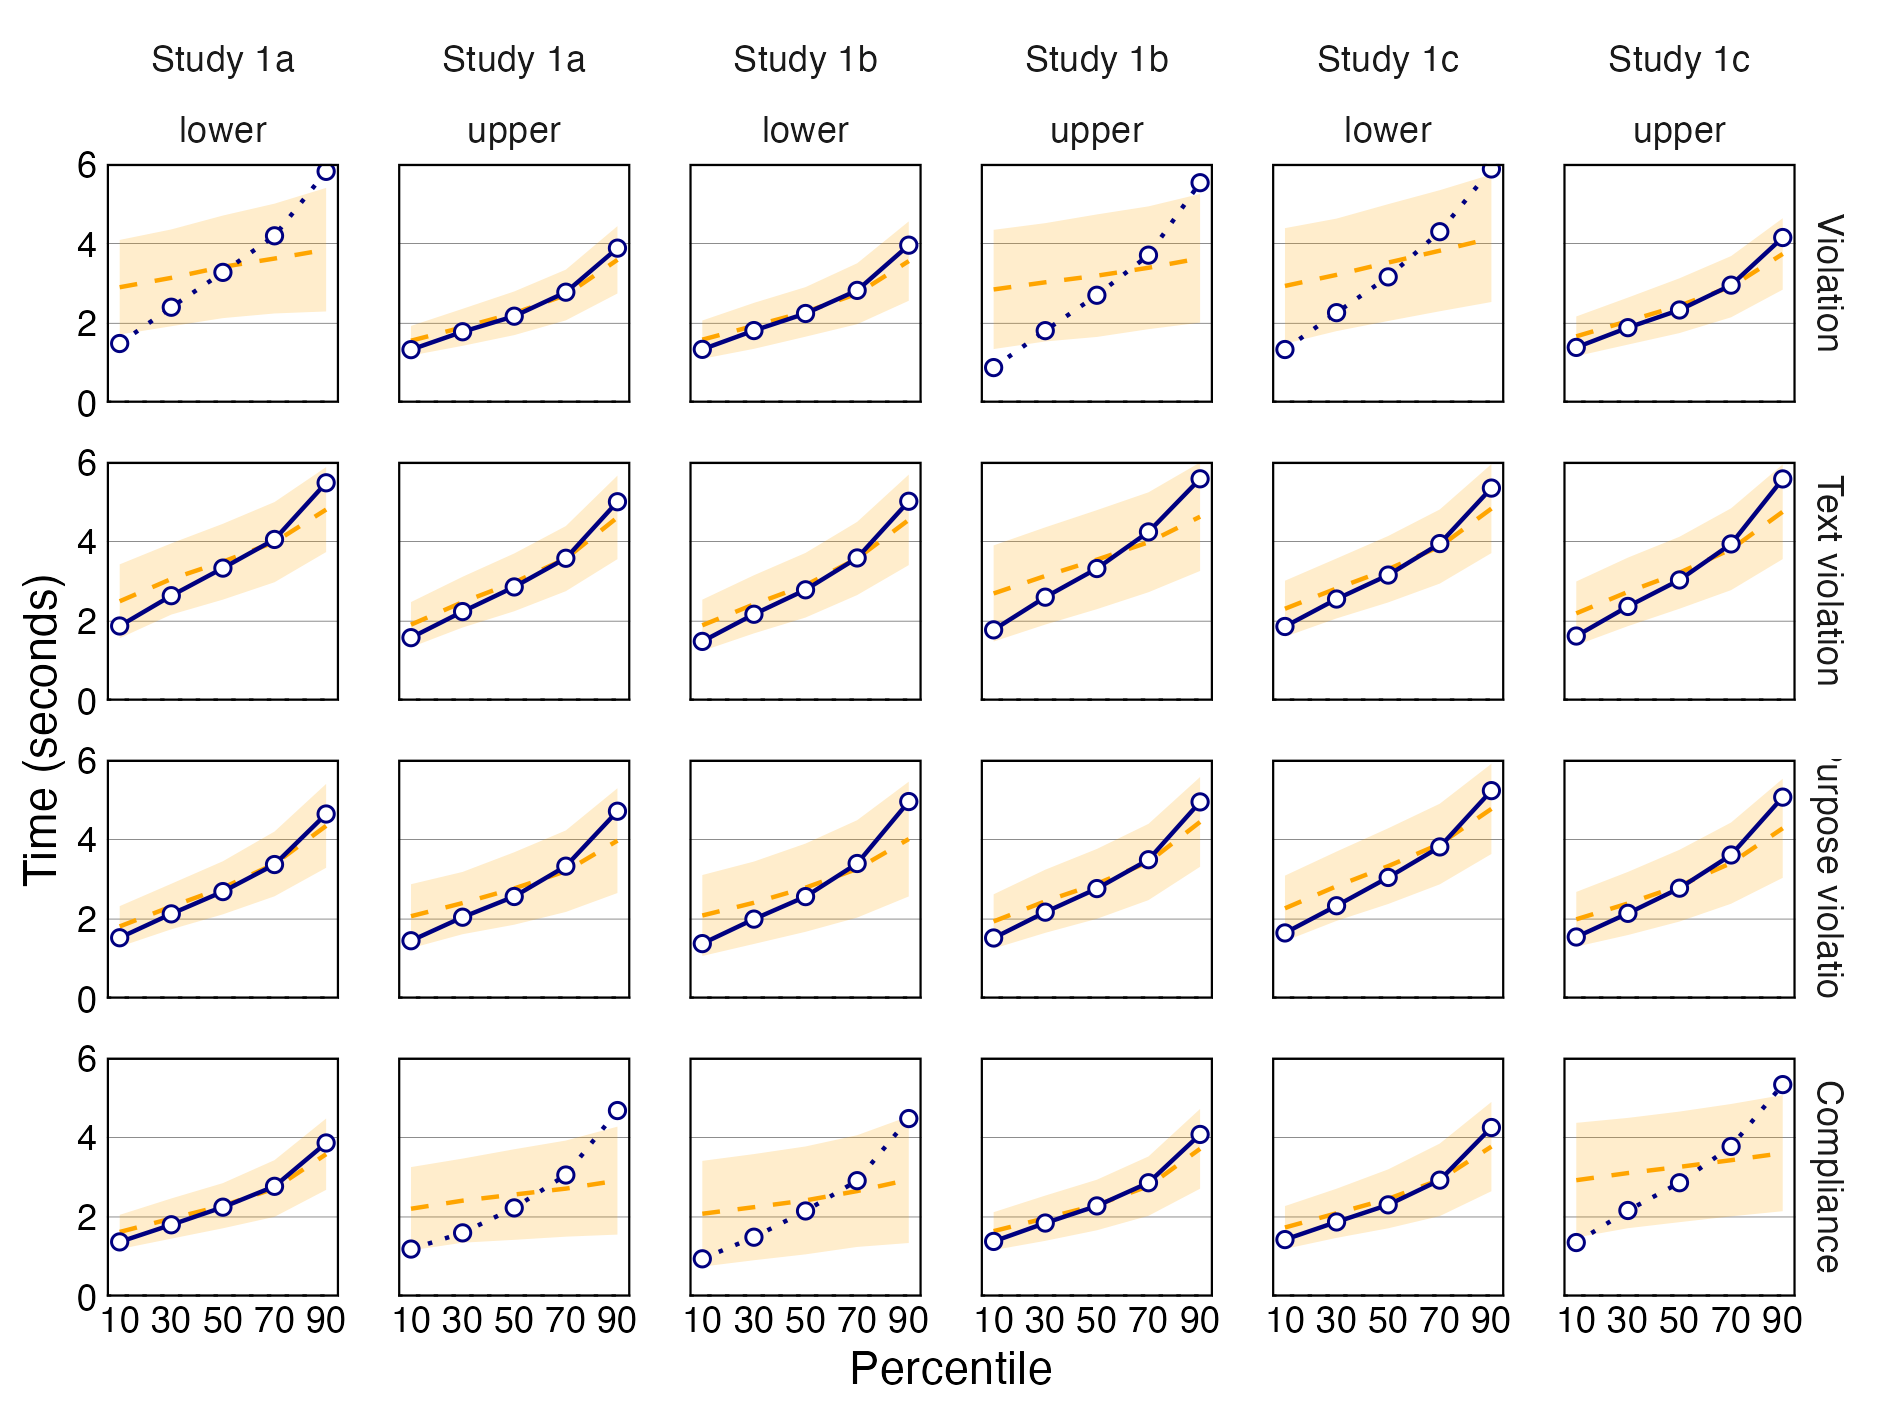
\includegraphics[width=\textwidth]{../figures/SuppFigure2.png}
  \caption{Observed reaction times (black) and 95\% confidence bands (orange), per study and response bound (columns) and case (rows): 10th, 30th, 50th, 70th, and 90th percentiles. Dotted lines indicate conditions representing erroneous responses in congruent cases.}
  \label{fig:S2}
\end{figure}

\clearpage

\FloatBarrier

% ============================================================
\subsection*{Supplementary Analysis 5: Bifactor model in Study 2}
\label{supp:analysis5}
% ============================================================

To examine whether individual differences in DDM parameters reflect task-general or task-specific processes, we conducted a series of bifactor confirmatory factor analyses. We first estimated a hierarchical DDM in which drift rate ($v$), threshold ($a$), and non-decision time ($t$) were each allowed to vary by task block, yielding four block-specific posterior means per parameter and participant. These individual-level estimates served as indicators in subsequent bifactor models.

For each DDM parameter, we specified a bifactor model comprising three task-specific factors (Flanker, Stroop, Rules) and one orthogonal general factor, with all indicators loading on both the common factor and their respective task-specific factor. All factors were constrained to be mutually orthogonal and standardized. Models were estimated via maximum likelihood using the lavaan package.

The bifactor model fit was excellent for non-decision time (CFI $= .999$, RMSEA $= .010$), threshold (CFI $= .991$, RMSEA $= .033$), and congruent drift rate (CFI $= 1.000$, RMSEA $= .000$). For the interference component of the drift rate, the bifactor model yielded an inadmissible solution, indicating that a general factor could not be extracted from interference scores. An orthogonal three-factor model fit well, and was not significantly worse than an oblique fit, $\Delta\chi^2(\mathit{df} = 3) = 4.44$, $p = .218$, confirming that the three task-specific conflict factors are mutually independent (see Supplementary Table~\ref{tab:S5}).

\begin{table}[h]
\caption{Model fit statistics for bifactor and orthogonal models (Study 2).}
\label{tab:S5}
\begin{tabular*}{\textwidth}{@{\extracolsep{\fill}}llrrrrrrr@{}}
\toprule
Parameter & Model & $\chi^2$ & $df$ & $p$ & CFI & TLI & RMSEA & SRMR \\
\midrule
Non-decision time ($t$)       & Bifactor           & 43.17 & 42 & .421 & .999 & .999 & .010 & .041 \\
Threshold ($a$)               & Bifactor           & 55.64 & 42 & .077 & .991 & .987 & .033 & .025 \\
Drift rate: congruent ($\beta_0$) & Bifactor       & 41.07 & 42 & .512 & 1.00 & 1.00 & .000 & .025 \\
Drift rate: interference ($\beta_1$) & Orthogonal  & 69.69 & 54 & .074 & .985 & .981 & .031 & .049 \\
\bottomrule
\end{tabular*}
\footnotetext{Model fit evaluated using: comparative fit index (CFI), Tucker--Lewis index (TLI), root mean square error of approximation (RMSEA) with 90\% CI, and standardized root mean square residual (SRMR). For the interference drift rate, the bifactor model yielded an inadmissible solution and was replaced by an orthogonal three-factor model. RMSEA 90\% CIs: $t$ [.000, .041]; $a$ [.000, .054]; $\beta_0$ [.000, .038]; $\beta_1$ [.000, .051].}
\end{table}


\clearpage

\FloatBarrier

% ============================================================
\subsection*{Supplementary Analysis 6: Logistic model of choice in Studies 3a--b}
\label{supp:analysis6}
% ============================================================

Supplementary Tables~\ref{tab:S6} and~\ref{tab:S7} report the results of mixed-effects logistic regression models of decisions in Studies 3a and 3b, with random intercepts of participant and scenario.

\begin{table}[htbp]
\caption{Mixed-effects logistic regression of decisions as a function of speed/accuracy condition, text, and purpose (Study 3a).}
\label{tab:S6}
\begin{tabular*}{\textwidth}{@{\extracolsep{\fill}}lrcrl@{}}
\toprule
Predictor & OR & 95\% CI & $z$ & $p$ \\
\midrule
(Intercept)                   & 0.06  & [0.05, 0.08]  & $-$22.31 & $<.001$ \\
Accuracy                      & 0.63  & [0.49, 0.81]  & $-$3.59  & $<.001$ \\
Text                          & 37.37 & [31.53, 44.30] & 41.74   & $<.001$ \\
Purpose                       & 5.89  & [4.98, 6.96]  & 20.80   & $<.001$ \\
Accuracy $\times$ Text        & 1.46  & [1.13, 1.87]  & 2.93    & .003    \\
Accuracy $\times$ Purpose     & 1.45  & [1.13, 1.86]  & 2.90    & .004    \\
\bottomrule
\end{tabular*}
\footnotetext{OR = odds ratio. Random effects: participants (SD = 0.416, ICC = .049, $N = 123$), rules (SD = 0.240, ICC = .016, $N = 8$). $N = 11{,}586$ observations. Pseudo-$R^2 = .568$ (fixed), $.596$ (total). AIC = 9407.27.}
\end{table}

\begin{table}[htbp]
\caption{Mixed-effects logistic regression of decisions as a function of congruency proportion, text, and purpose (Study 3b).}
\label{tab:S7}
\begin{tabular*}{\textwidth}{@{\extracolsep{\fill}}lrcrl@{}}
\toprule
Predictor & OR & 95\% CI & $z$ & $p$ \\
\midrule
(Intercept)                      & 0.04  & [0.03, 0.05]  & $-$17.70 & $<.001$ \\
Congruency                       & 0.77  & [0.55, 1.07]  & $-$1.56  & .120    \\
Text                             & 53.49 & [40.68, 70.35] & 28.48   & $<.001$ \\
Purpose                          & 5.64  & [4.31, 7.38]  & 12.63   & $<.001$ \\
Congruency $\times$ Text         & 1.56  & [1.11, 2.20]  & 2.56    & .011    \\
Congruency $\times$ Purpose      & 1.53  & [1.09, 2.14]  & 2.45    & .014    \\
\bottomrule
\end{tabular*}
\footnotetext{OR = odds ratio. Random effects: participants (SD = 0.416, ICC = .049, $N = 121$), rules (SD = 0.240, ICC = .016, $N = 8$). $N = 11{,}586$ observations. Pseudo-$R^2 = .568$ (fixed), $.596$ (total). AIC = 9407.27.}
\end{table}

\clearpage

\FloatBarrier

% ============================================================
\subsection*{Supplementary Analysis 7: Log-linear model of reaction times in Studies 3a--b}
\label{supp:analysis7}
% ============================================================

A linear regression model of reaction times revealed a main effect of accuracy mode, which was qualified by higher-order interactions (see Supplementary Table~\ref{tab:S8}). Decomposition of the three-way interaction revealed that participants availed themselves of more additional time to resolve incongruent ($\Delta\mathrm{RT} = 816$--$1009$~ms) than congruent ($\Delta\mathrm{RT} = 597$--$655$~ms) cases, $t$s $> 2.89$, $p$s $< .020$.

A log-linear regression model of reaction times revealed no main effect of congruency proportion, but two- and three-way interactions with text and purpose, $p$s $< .001$---confirming the proportion of congruency effect on reaction times. Specifically, the three-way interaction revealed that responses to congruent trials were faster than responses to incongruent trials in both congruency proportion blocks, but the median difference was larger when incongruent trials were rare ($\Delta\mathrm{RT} = 822$~ms) than when they were frequent ($\Delta\mathrm{RT} = 395$~ms; see Supplementary Table~\ref{tab:S9}).

\begin{table}[htbp]
\caption{Mixed-effects linear regression predicting log reaction time as a function of speed/accuracy condition, text, and purpose (Study 3a).}
\label{tab:S8}
\begin{tabular*}{\textwidth}{@{\extracolsep{\fill}}lrcrl@{}}
\toprule
Predictor & $B$ & 95\% CI & $t$ & $p$ \\
\midrule
(Intercept)                              & 7.610 & [7.533, 7.688] & 192.86  & $<.001$ \\
Accuracy                                 & 0.210 & [0.184, 0.235] & 15.84   & $<.001$ \\
Text                                     & 0.173 & [0.147, 0.199] & 12.99   & $<.001$ \\
Purpose                                  & 0.120 & [0.094, 0.146] & 9.08    & $<.001$ \\
Text $\times$ Purpose                    & $-$0.295 & [$-$0.332, $-$0.258] & $-$15.73 & $<.001$ \\
Accuracy $\times$ Text                   & 0.088 & [0.051, 0.125] & 4.71    & $<.001$ \\
Accuracy $\times$ Purpose                & 0.043 & [0.006, 0.079] & 2.27    & .023    \\
Accuracy $\times$ Text $\times$ Purpose  & $-$0.111 & [$-$0.163, $-$0.059] & $-$4.20 & $<.001$ \\
\bottomrule
\end{tabular*}
\footnotetext{$p$ values computed using Satterthwaite degrees of freedom. Random effects: participants (SD = 0.201, ICC = .230, $N = 123$), rules (SD = 0.096, ICC = .052, $N = 8$), residual SD = 0.356. $N = 11{,}586$ observations. Pseudo-$R^2 = .119$ (fixed), $.367$ (total). AIC = 9482.93.}
\end{table}

\begin{table}[htbp]
\caption{Mixed-effects linear regression predicting log response time as a function of congruency proportion, text, and purpose (Study 3b).}
\label{tab:S9}
\begin{tabular*}{\textwidth}{@{\extracolsep{\fill}}lrcrl@{}}
\toprule
Predictor & $B$ & 95\% CI & $t$ & $p$ \\
\midrule
(Intercept)                                    & 7.725 & [7.634, 7.816] & 165.78  & $<.001$ \\
Congruency                                     & $-$0.073 & [$-$0.109, $-$0.036] & $-$3.90 & $<.001$ \\
Text                                           & 0.209 & [0.173, 0.246] & 11.22   & $<.001$ \\
Purpose                                        & 0.120 & [0.084, 0.157] & 6.45    & $<.001$ \\
Text $\times$ Purpose                          & $-$0.266 & [$-$0.318, $-$0.215] & $-$10.09 & $<.001$ \\
Congruency $\times$ Text                       & 0.058 & [0.006, 0.110] & 2.20    & .028    \\
Congruency $\times$ Purpose                    & 0.190 & [0.139, 0.242] & 7.21    & $<.001$ \\
Congruency $\times$ Text $\times$ Purpose      & $-$0.301 & [$-$0.374, $-$0.228] & $-$8.06 & $<.001$ \\
\bottomrule
\end{tabular*}
\footnotetext{$p$ values computed using Satterthwaite degrees of freedom. Random effects: participants (SD = 0.292, ICC = .365, $N = 121$), rules (SD = 0.097, ICC = .040, $N = 8$), residual SD = 0.373. $N = 11{,}482$ observations. Pseudo-$R^2 = .058$ (fixed), $.440$ (total). AIC = 10550.93.}
\end{table}

\clearpage

\FloatBarrier

% ============================================================
\subsection*{Supplementary Analysis 8: Drift diffusion models in Studies 3a--b}
\label{supp:analysis8}
% ============================================================

Supplementary Tables~\ref{tab:S10} and~\ref{tab:S11} report the results of the hddmRegressor models in Studies 3a and 3b. The accuracy and congruency proportion manipulations moderated the drift rates of text and purpose in the same direction---resulting in no overall change on incongruent trials.

\begin{table}[htbp]
\caption{Drift diffusion model parameter estimates (Study 3a).}
\label{tab:S10}
\begin{tabular*}{\textwidth}{@{\extracolsep{\fill}}llrr@{}}
\toprule
Parameter & Predictor & $M$ & 95\% HDI \\
\midrule
\multirow{6}{*}{Drift rate ($v$)} & Intercept & $-$1.211 & [$-$1.283, $-$1.138] \\
 & Text                      & 1.481  & [1.384, 1.579]   \\
 & Speed (vs.\ Accuracy)     & $-$0.064 & [$-$0.140, 0.016] \\
 & Purpose                   & 0.720  & [0.648, 0.795]   \\
 & Text $\times$ Speed       & 0.173  & [0.083, 0.261]   \\
 & Purpose $\times$ Speed    & 0.003  & [$-$0.076, 0.081] \\
\midrule
\multirow{2}{*}{Threshold ($a$)} & Intercept & 3.425 & [3.322, 3.535] \\
 & Speed (vs.\ Accuracy)     & $-$0.647 & [$-$0.760, $-$0.532] \\
\midrule
\multirow{2}{*}{Non-decision time ($t$)} & Intercept & 1.135 & [1.065, 1.209] \\
 & Speed (vs.\ Accuracy)     & $-$0.084 & [$-$0.148, $-$0.019] \\
\midrule
\multirow{2}{*}{Bias ($z$)} & Intercept & 0.531 & [0.519, 0.543] \\
 & Speed (vs.\ Accuracy)     & $-$0.007 & [$-$0.024, 0.011] \\
\bottomrule
\end{tabular*}
\footnotetext{Estimates are posterior means with 95\% highest density intervals from HDDM. Predictors coded as dummy variables; reference category is accuracy condition, no-text, no-purpose.}
\end{table}

\begin{table}[htbp]
\caption{Drift diffusion model parameter estimates (Study 3b).}
\label{tab:S11}
\begin{tabular*}{\textwidth}{@{\extracolsep{\fill}}llrr@{}}
\toprule
Parameter & Predictor & $M$ & 95\% HDI \\
\midrule
\multirow{6}{*}{Drift rate ($v$)} & Intercept & $-$1.293 & [$-$1.379, $-$1.210] \\
 & Text                                  & 1.537  & [1.431, 1.645]   \\
 & Congruency: high (vs.\ low)           & $-$0.123 & [$-$0.209, $-$0.040] \\
 & Purpose                               & 0.575  & [0.497, 0.652]   \\
 & Text $\times$ Congruency              & 0.234  & [0.128, 0.334]   \\
 & Purpose $\times$ Congruency           & 0.268  & [0.197, 0.350]   \\
\midrule
\multirow{2}{*}{Threshold ($a$)} & Intercept & 3.076 & [2.965, 3.191] \\
 & Congruency: high (vs.\ low)           & 0.490  & [0.349, 0.642]   \\
\midrule
\multirow{2}{*}{Non-decision time ($t$)} & Intercept & 1.128 & [1.049, 1.211] \\
 & Congruency: high (vs.\ low)           & $-$0.215 & [$-$0.273, $-$0.158] \\
\midrule
\multirow{2}{*}{Bias ($z$)} & Intercept & 0.532 & [0.520, 0.544] \\
 & Congruency: high (vs.\ low)           & $-$0.001 & [$-$0.016, 0.016] \\
\bottomrule
\end{tabular*}
\footnotetext{Estimates are posterior means with 95\% highest density intervals from HDDM. Reference category is high congruency condition, no-text, no-purpose.}
\end{table}

\clearpage

\FloatBarrier

% ============================================================
\subsection*{Supplementary Analysis 9: Interim analysis of trial number effects in Studies 1a--3b}
\label{supp:analysis9}
% ============================================================

As exploratory evidence of an adaptation effect, we jointly analyzed 85,819 responses from 909 participants across the first six studies. To aggregate across different dependent measures, we reverse-scored compliance judgments in Experiment 1b and called this new measure \textit{judgment}, where 1 = conviction and 0 = acquittal. In the mixed-effects model of judgments, we found a stronger effect of text as a function of trial number, $\mathrm{OR}_\text{Trial$\times$Text} = 1.78$, 95\% CI $[1.52, 2.09]$, $z = 7.08$, $p < .001$, but no difference in the effect of purpose, $\mathrm{OR}_\text{Trial$\times$Purpose} = 0.91$, 95\% CI $[0.77, 1.06]$, $z = -1.21$, $p = .23$ (see Supplementary Table~\ref{tab:S12}).

\begin{sidewaystable}
\caption{Mega-analysis of Studies 1a--3b: Mixed-effects logistic regression models of rule interpretation across studies.}
\label{tab:S12}
\begin{tabular*}{\textheight}{@{\extracolsep{\fill}}lrcrllrcrl@{}}
\toprule
 & \multicolumn{4}{c}{Model 1} & & \multicolumn{4}{c}{Model 2} \\
\cmidrule{2-5} \cmidrule{7-10}
Predictor & OR & 95\% CI & $z$ & $p$ & & OR & 95\% CI & $z$ & $p$ \\
\midrule
(Intercept)              & 0.063 & [0.048, 0.083] & $-$19.97 & $<.001$ && 0.218 & [0.133, 0.356] & $-$6.08 & $<.001$ \\
Trial ($z$)              & 0.768 & [0.654, 0.901] & $-$3.24  & .001   && 0.772 & [0.658, 0.907] & $-$3.15 & .002   \\
Text                     & 30.314& [27.699, 33.175]& 74.13  & $<.001$ && 11.065& [6.999, 17.495]& 10.29  & $<.001$ \\
Purpose                  & 7.859 & [7.186, 8.594] & 45.17   & $<.001$ && 1.925 & [1.220, 3.036] & 2.82   & .005   \\
Limit                    & 0.984 & [0.965, 1.004] & $-$1.54  & .124   && 0.911 & [0.868, 0.956] & $-$3.79 & $<.001$ \\
Proportion               & 1.371 & [1.166, 1.612] & 3.82    & $<.001$ && 0.602 & [0.394, 0.919] & $-$2.35 & .019   \\
DV: punishment           & 0.740 & [0.657, 0.834] & $-$4.94  & $<.001$ && 0.663 & [0.546, 0.804] & $-$4.17 & $<.001$ \\
DV: violate              & 0.822 & [0.750, 0.900] & $-$4.21  & $<.001$ && 0.630 & [0.544, 0.730] & $-$6.15 & $<.001$ \\
Trial $\times$ Text      & 1.779 & [1.517, 2.087] & 7.08    & $<.001$ && 1.804 & [1.537, 2.118] & 7.21   & $<.001$ \\
Trial $\times$ Purpose   & 0.906 & [0.773, 1.063] & $-$1.21  & .225   && 0.885 & [0.754, 1.038] & $-$1.50 & .133   \\
Limit $\times$ Text      & ---   & ---            & ---     & ---    && 1.086 & [1.034, 1.139] & 3.33   & .001   \\
Limit $\times$ Purpose   & ---   & ---            & ---     & ---    && 1.067 & [1.017, 1.120] & 2.65   & .008   \\
Proportion $\times$ Text & ---   & ---            & ---     & ---    && 1.871 & [1.233, 2.840] & 2.94   & .003   \\
Proportion $\times$ Purpose & --- & ---           & ---     & ---    && 2.821 & [1.864, 4.271] & 4.90   & $<.001$ \\
Punishment $\times$ Text & ---   & ---            & ---     & ---    && 0.368 & [0.311, 0.435] & $-$11.67 & $<.001$ \\
Violate $\times$ Text    & ---   & ---            & ---     & ---    && 1.273 & [1.117, 1.451] & 3.62   & $<.001$ \\
Punishment $\times$ Purpose & --- & ---           & ---     & ---    && 3.639 & [3.078, 4.302] & 15.13  & $<.001$ \\
Violate $\times$ Purpose & ---   & ---            & ---     & ---    && 1.296 & [1.139, 1.475] & 3.93   & $<.001$ \\
\midrule
$N$ (observations)       & \multicolumn{4}{l}{85,819} && \multicolumn{4}{l}{85,819} \\
$N$ (subjects)           & \multicolumn{4}{l}{909}    && \multicolumn{4}{l}{909}    \\
$N$ (rules)              & \multicolumn{4}{l}{8}      && \multicolumn{4}{l}{8}      \\
Pseudo-$R^2$ (fixed)     & \multicolumn{4}{l}{.561}   && \multicolumn{4}{l}{.569}   \\
Pseudo-$R^2$ (total)     & \multicolumn{4}{l}{.586}   && \multicolumn{4}{l}{.595}   \\
AIC                      & \multicolumn{4}{l}{70749.63} && \multicolumn{4}{l}{69266.72} \\
\bottomrule
\end{tabular*}
\footnotetext{OR = odds ratio. Reference category for DV is acquit. Model 2 adds interactions of all covariates with text and purpose. Non-significant predictors ($p > .05$): Limit in Model 1, Trial $\times$ Purpose in both models.}
\end{sidewaystable}

\clearpage

\FloatBarrier

% ============================================================
\subsection*{Supplementary Analysis 10: Logistic model of choice in Studies 4a--b}
\label{supp:analysis10}
% ============================================================

Supplementary Tables~\ref{tab:S13} and~\ref{tab:S14} report the results of mixed-effects logistic regression models of decisions in Study 4a, allowing (raw) trial number and log-trial number, respectively, to moderate the effects of text and purpose. Supplementary Table~\ref{tab:S15} describes the pattern of block-level comparisons (Executive Demand vs.\ Task Experience). The patterns of pre-to-post change in Study 4b are described in Supplementary Tables~\ref{tab:S16}--\ref{tab:S18}, separately for each level of the between-subjects treatment.

\begin{table}[htbp]
\caption{Trial effects in Study 4a.}
\label{tab:S13}
\begin{tabular*}{\textwidth}{@{\extracolsep{\fill}}lrcrl@{}}
\toprule
Predictor & OR & 95\% CI & $z$ & $p$ \\
\midrule
(Intercept)                  & 0.197 & [0.159, 0.245] & $-$14.66 & $<.001$ \\
Trial                        & 0.876 & [0.672, 1.143] & $-$0.98  & .330    \\
Text                         & 9.060 & [7.831, 10.482] & 29.63  & $<.001$ \\
Purpose                      & 4.155 & [3.595, 4.803] & 19.26   & $<.001$ \\
Trial $\times$ Text          & 1.438 & [1.079, 1.917] & 2.48    & .013    \\
Trial $\times$ Purpose       & 0.748 & [0.562, 0.997] & $-$1.98  & .047    \\
\bottomrule
\end{tabular*}
\footnotetext{OR = odds ratio. Random effects: participants (SD = 0.314, ICC = .029, $N = 227$), rules (SD = 0.241, ICC = .017, $N = 8$). $N = 15{,}656$ observations. Pseudo-$R^2 = .346$ (fixed), $.376$ (total). AIC = 16,570.01.}
\end{table}

\begin{table}[htbp]
\caption{Log-trial effects in Study 4a.}
\label{tab:S14}
\begin{tabular*}{\textwidth}{@{\extracolsep{\fill}}lrcrl@{}}
\toprule
Predictor & OR & 95\% CI & $z$ & $p$ \\
\midrule
(Intercept)                      & 0.186 & [0.155, 0.225] & $-$17.60 & $<.001$ \\
$\log(\text{Trial})$             & 0.943 & [0.874, 1.017] & $-$1.53  & .127    \\
Text                             & 10.565& [9.747, 11.451] & 57.38  & $<.001$ \\
Purpose                          & 3.677 & [3.397, 3.980] & 32.20   & $<.001$ \\
$\log(\text{Trial}) \times$ Text & 1.134 & [1.043, 1.233] & 2.95    & .003    \\
$\log(\text{Trial}) \times$ Purpose & 0.925 & [0.851, 1.005] & $-$1.83 & .067 \\
\bottomrule
\end{tabular*}
\footnotetext{OR = odds ratio. Trial was log-transformed and mean-centered prior to analysis; the intercept represents odds at the average trial. Random effects: participants (SD = 0.313, ICC = .028, $N = 227$), rules (SD = 0.241, ICC = .017, $N = 8$). $N = 15{,}656$ observations. Pseudo-$R^2 = .346$ (fixed), $.376$ (total). AIC = 16,566.60.}
\end{table}

\begin{table}[htbp]
\caption{Block-level effect in Study 4a.}
\label{tab:S15}
\begin{tabular*}{\textwidth}{@{\extracolsep{\fill}}lrcrl@{}}
\toprule
Predictor & OR & 95\% CI & $z$ & $p$ \\
\midrule
(Intercept)                        & 0.207 & [0.167, 0.256] & $-$14.49 & $<.001$ \\
Task Experience                      & 0.883 & [0.743, 1.048] & $-$1.42  & .156    \\
Executive Demand                     & 0.833 & [0.685, 1.013] & $-$1.83  & .067    \\
Text                               & 9.173 & [8.028, 10.481] & 32.59  & $<.001$ \\
Purpose                            & 3.951 & [3.461, 4.510] & 20.34   & $<.001$ \\
Task Experience $\times$ Text        & 1.250 & [1.034, 1.511] & 2.31    & .021    \\
Executive Demand $\times$ Text       & 1.239 & [1.019, 1.506] & 2.15    & .032    \\
Task Experience $\times$ Purpose     & 0.859 & [0.711, 1.037] & $-$1.58  & .11     \\
Executive Demand $\times$ Purpose    & 0.935 & [0.770, 1.136] & $-$0.68  & .50     \\
\bottomrule
\end{tabular*}
\footnotetext{OR = odds ratio. Reference category: Block 1 (Rules$_0$). Random effects: participants (SD = 0.311, ICC = .028, $N = 227$), rules (SD = 0.241, ICC = .017, $N = 8$). $N = 15{,}656$ observations. Pseudo-$R^2 = .347$ (fixed), $.376$ (total). AIC = 16,574.27.}
\end{table}

\begin{table}[htbp]
\caption{Pre-to-post change: Passive Control treatment (Study 4b).}
\label{tab:S16}
\begin{tabular*}{\textwidth}{@{\extracolsep{\fill}}lrcrl@{}}
\toprule
Predictor & OR & 95\% CI & $z$ & $p$ \\
\midrule
(Intercept)                & 0.064 & [0.049, 0.085] & $-$19.45 & $<.001$ \\
Post-Block                 & 0.918 & [0.719, 1.172] & $-$0.69  & .493    \\
Text                       & 19.775& [16.539, 23.644]& 32.73  & $<.001$ \\
Purpose                    & 11.346& [9.504, 13.546] & 26.86  & $<.001$ \\
Post-Block $\times$ Text   & 1.254 & [0.977, 1.609] & 1.78    & .075    \\
Post-Block $\times$ Purpose& 0.848 & [0.662, 1.088] & $-$1.30  & .195    \\
\bottomrule
\end{tabular*}
\footnotetext{OR = odds ratio. Random effects: participants (SD = 0.466, ICC = .061, $N = 205$), rules (SD = 0.297, ICC = .025, $N = 8$). $N = 9{,}854$ observations. Pseudo-$R^2 = .518$ (fixed), $.559$ (total). AIC = 8,896.57.}
\end{table}

\begin{table}[htbp]
\caption{Pre-to-post change: Executive Demand treatment (Study 4b).}
\label{tab:S17}
\begin{tabular*}{\textwidth}{@{\extracolsep{\fill}}lrcrl@{}}
\toprule
Predictor & OR & 95\% CI & $z$ & $p$ \\
\midrule
(Intercept)                & 0.072 & [0.054, 0.095] & $-$18.39 & $<.001$ \\
Post-Block                 & 1.078 & [0.858, 1.355] & 0.64    & .521    \\
Text                       & 17.942& [15.142, 21.260]& 33.35  & $<.001$ \\
Purpose                    & 9.150 & [7.738, 10.820] & 25.88  & $<.001$ \\
Post-Block $\times$ Text   & 1.331 & [1.052, 1.683] & 2.39    & .017    \\
Post-Block $\times$ Purpose& 0.662 & [0.524, 0.836] & $-$3.46  & $<.001$ \\
\bottomrule
\end{tabular*}
\footnotetext{OR = odds ratio. Random effects: participants (SD = 0.304, ICC = .027, $N = 209$), rules (SD = 0.322, ICC = .030, $N = 8$). $N = 10{,}012$ observations. Pseudo-$R^2 = .494$ (fixed), $.522$ (total). AIC = 9,209.28.}
\end{table}

\begin{table}[htbp]
\caption{Pre-to-post change: Task Experience treatment (Study 4b).}
\label{tab:S18}
\begin{tabular*}{\textwidth}{@{\extracolsep{\fill}}lrcrl@{}}
\toprule
Predictor & OR & 95\% CI & $z$ & $p$ \\
\midrule
(Intercept)                & 0.058 & [0.044, 0.077] & $-$19.92 & $<.001$ \\
Post-Block                 & 1.255 & [0.973, 1.618] & 1.75    & .080    \\
Text                       & 24.404& [20.093, 29.640]& 32.21  & $<.001$ \\
Purpose                    & 11.108& [9.161, 13.470] & 24.48  & $<.001$ \\
Post-Block $\times$ Text   & 0.895 & [0.690, 1.160] & $-$0.84  & .401    \\
Post-Block $\times$ Purpose& 0.617 & [0.476, 0.799] & $-$3.66  & $<.001$ \\
\bottomrule
\end{tabular*}
\footnotetext{OR = odds ratio. Random effects: participants (SD = 0.356, ICC = .036, $N = 186$), rules (SD = 0.288, ICC = .024, $N = 8$). $N = 8{,}941$ observations. Pseudo-$R^2 = .516$ (fixed), $.545$ (total). AIC = 8,084.08.}
\end{table}

\clearpage

\FloatBarrier

% ============================================================
\subsection*{Supplementary Analysis 11: Drift diffusion models in Studies 4a--b}
\label{supp:analysis11}
% ============================================================
Supplementary Tables~\ref{tab:S19}--\ref{tab:S22} report the results of the hddmRegressor models in Studies 4a and 4b. Studies 4a and 4b revealed consistent increases in the drift rate of text as a result of Task Experience and Executive Demand.

\begin{table}[htbp]
\caption{Drift diffusion model parameter estimates (Study 4a).}
\label{tab:S19}
\begin{tabular*}{\textwidth}{@{\extracolsep{\fill}}llrr@{}}
\toprule
Parameter & Predictor & $M$ & 95\% HDI \\
\midrule
\multirow{9}{*}{Drift rate ($v$)} & Intercept & $-$0.626 & [$-$0.667, $-$0.584] \\
 & Text                              & 0.843  & [0.797, 0.888]   \\
 & Purpose                           & 0.496  & [0.456, 0.539]   \\
 & Rules$_E$                         & $-$0.114 & [$-$0.171, $-$0.059] \\
 & Rules$_D$                         & $-$0.095 & [$-$0.157, $-$0.034] \\
 & Text $\times$ Rules$_E$           & 0.144  & [0.079, 0.211]   \\
 & Text $\times$ Rules$_D$           & 0.107  & [0.039, 0.174]   \\
 & Purpose $\times$ Rules$_E$        & $-$0.023 & [$-$0.087, 0.041] \\
 & Purpose $\times$ Rules$_D$        & $-$0.009 & [$-$0.072, 0.054] \\
\midrule
\multirow{3}{*}{Threshold ($a$)} & Intercept & 3.050 & [2.941, 3.156] \\
 & Rules$_E$                         & $-$0.210 & [$-$0.268, $-$0.146] \\
 & Rules$_D$                         & $-$0.106 & [$-$0.263, 0.061]  \\
\midrule
\multirow{3}{*}{Non-decision time ($t$)} & Intercept & 1.373 & [1.256, 1.501] \\
 & Rules$_E$                         & $-$0.037 & [$-$0.060, $-$0.015] \\
 & Rules$_D$                         & $-$0.062 & [$-$0.152, 0.007]  \\
\midrule
Bias ($z$) & Intercept & 0.532 & [0.524, 0.540] \\
\bottomrule
\end{tabular*}
\footnotetext{Rules$_0$ = baseline block (reference); Rules$_E$ = Task Experience block; Rules$_D$ = Executive Demand block.}
\end{table}

\begin{table}[htbp]
\caption{Drift diffusion model parameter estimates (Study 4b: Passive Control).}
\label{tab:S20}
\begin{tabular*}{\textwidth}{@{\extracolsep{\fill}}llrr@{}}
\toprule
Parameter & Predictor & $M$ & 95\% HDI \\
\midrule
\multirow{5}{*}{Drift rate ($v$)} & Intercept & $-$0.985 & [$-$1.052, $-$0.928] \\
 & Text                              & 1.043  & [0.970, 1.109]   \\
 & Purpose                           & 0.851  & [0.781, 0.918]   \\
 & Post-Block                        & $-$0.248 & [$-$0.325, $-$0.174] \\
 & Text $\times$ Post-Block          & 0.306  & [0.215, 0.392]   \\
 & Purpose $\times$ Post-Block       & 0.087  & [0.005, 0.173]   \\
\midrule
\multirow{2}{*}{Threshold ($a$)} & Intercept & 3.074 & [2.991, 3.168] \\
 & Post-Block                        & $-$0.059 & [$-$0.159, 0.033] \\
\midrule
\multirow{2}{*}{Non-decision time ($t$)} & Intercept & 1.398 & [1.313, 1.493] \\
 & Post-Block                        & $-$0.031 & [$-$0.084, 0.023] \\
\midrule
Bias ($z$) & Intercept & 0.537 & [0.528, 0.546] \\
\bottomrule
\end{tabular*}
\end{table}

\begin{table}[htbp]
\caption{Drift diffusion model parameter estimates (Study 4b: Executive Demand).}
\label{tab:S21}
\begin{tabular*}{\textwidth}{@{\extracolsep{\fill}}llrr@{}}
\toprule
Parameter & Predictor & $M$ & 95\% HDI \\
\midrule
\multirow{6}{*}{Drift rate ($v$)} & Intercept & $-$0.976 & [$-$1.029, $-$0.924] \\
 & Text                              & 1.023  & [0.952, 1.095]   \\
 & Purpose                           & 0.763  & [0.695, 0.828]   \\
 & Post-Block                        & $-$0.125 & [$-$0.195, $-$0.063] \\
 & Text $\times$ Post-Block          & 0.302  & [0.218, 0.387]   \\
 & Purpose $\times$ Post-Block       & $-$0.054 & [$-$0.135, 0.025] \\
\midrule
\multirow{2}{*}{Threshold ($a$)} & Intercept & 3.073 & [2.996, 3.159] \\
 & Post-Block                        & $-$0.119 & [$-$0.203, $-$0.028] \\
\midrule
\multirow{2}{*}{Non-decision time ($t$)} & Intercept & 1.457 & [1.376, 1.540] \\
 & Post-Block                        & $-$0.189 & [$-$0.248, $-$0.131] \\
\midrule
Bias ($z$) & Intercept & 0.547 & [0.538, 0.557] \\
\bottomrule
\end{tabular*}
\end{table}

\begin{table}[htbp]
\caption{Drift diffusion model parameter estimates (Study 4b: Task Experience).}
\label{tab:S22}
\begin{tabular*}{\textwidth}{@{\extracolsep{\fill}}llrr@{}}
\toprule
Parameter & Predictor & $M$ & 95\% HDI \\
\midrule
\multirow{6}{*}{Drift rate ($v$)} & Intercept & $-$0.996 & [$-$1.053, $-$0.944] \\
 & Text                              & 1.108  & [1.031, 1.189]   \\
 & Purpose                           & 0.802  & [0.730, 0.869]   \\
 & Post-Block                        & $-$0.141 & [$-$0.210, $-$0.069] \\
 & Text $\times$ Post-Block          & 0.197  & [0.110, 0.280]   \\
 & Purpose $\times$ Post-Block       & $-$0.014 & [$-$0.102, 0.082] \\
\midrule
\multirow{2}{*}{Threshold ($a$)} & Intercept & 3.126 & [3.041, 3.220] \\
 & Post-Block                        & $-$0.161 & [$-$0.249, $-$0.067] \\
\midrule
\multirow{2}{*}{Non-decision time ($t$)} & Intercept & 1.408 & [1.304, 1.515] \\
 & Post-Block                        & $-$0.191 & [$-$0.256, $-$0.124] \\
\midrule
Bias ($z$) & Intercept & 0.532 & [0.521, 0.542] \\
\bottomrule
\end{tabular*}
\end{table}

\end{appendices}

\end{document}
